\documentclass[times, utf8, zavrsni]{fer}
\usepackage{booktabs}


\usepackage[croatian]{babel} 
\usepackage{amssymb}
\usepackage{amsmath}
\usepackage{txfonts}
\usepackage{mathdots}
\usepackage{titlesec}
\usepackage{array}
\usepackage{lastpage}
\usepackage{etoolbox}
\usepackage{tabularray}
\usepackage{color, colortbl}
\usepackage{adjustbox}
\usepackage{geometry}
\usepackage[classicReIm]{kpfonts}
\usepackage{hyperref}
\usepackage{fancyhdr}
\usepackage[T1]{fontenc}     % default is 'OT1'
\usepackage[utf8]{inputenc}
\usepackage{graphicx}

\usepackage{float}
\usepackage{setspace}

\usepackage{pdfpages}
\restylefloat{table}


%boja za privatni i udaljeni kljuc u tablicama
\definecolor{LightBlue}{rgb}{0.9,0.9,1}
\definecolor{LightGreen}{rgb}{0.9,1,0.9}

%Promjena teksta za dugačke tablice
\DefTblrTemplate{contfoot-text}{normal}{Nastavljeno na idućoj stranici}
\SetTblrTemplate{contfoot-text}{normal}
\DefTblrTemplate{conthead-text}{normal}{(Nastavljeno)}
\SetTblrTemplate{conthead-text}{normal}
\DefTblrTemplate{middlehead,lasthead}{normal}{Nastavljeno od prethodne stranice}
\SetTblrTemplate{middlehead,lasthead}{normal}


%Programski kod
\usepackage{courier} %% Sets font for listing as Courier.
\usepackage{listings, xcolor}
\lstset{
tabsize = 4, %% set tab space width
showstringspaces = false, %% prevent space marking in strings, string is defined as the text that is generally printed directly to the console
numbers = left, %% display line numbers on the left
commentstyle = \color{green}, %% set comment color
keywordstyle = \color{blue}, %% set keyword color
stringstyle = \color{red}, %% set string color
rulecolor = \color{black}, %% set frame color to avoid being affected by text color
basicstyle = \scriptsize \ttfamily , %% set listing font and size
breaklines = true, %% enable line breaking
numberstyle = \tiny,
}




\begin{document}

% TODO: Navedite broj rada.
\thesisnumber{663}

% TODO: Navedite naslov rada.
\title{Mobilna igra za vježbanje matematike}

% TODO: Navedite vaše ime i prezime.
\author{Denis Pipalović}

\maketitle

% Ispis stranice s napomenom o umetanju izvornika rada. Uklonite naredbu \izvornik ako želite izbaciti tu stranicu.
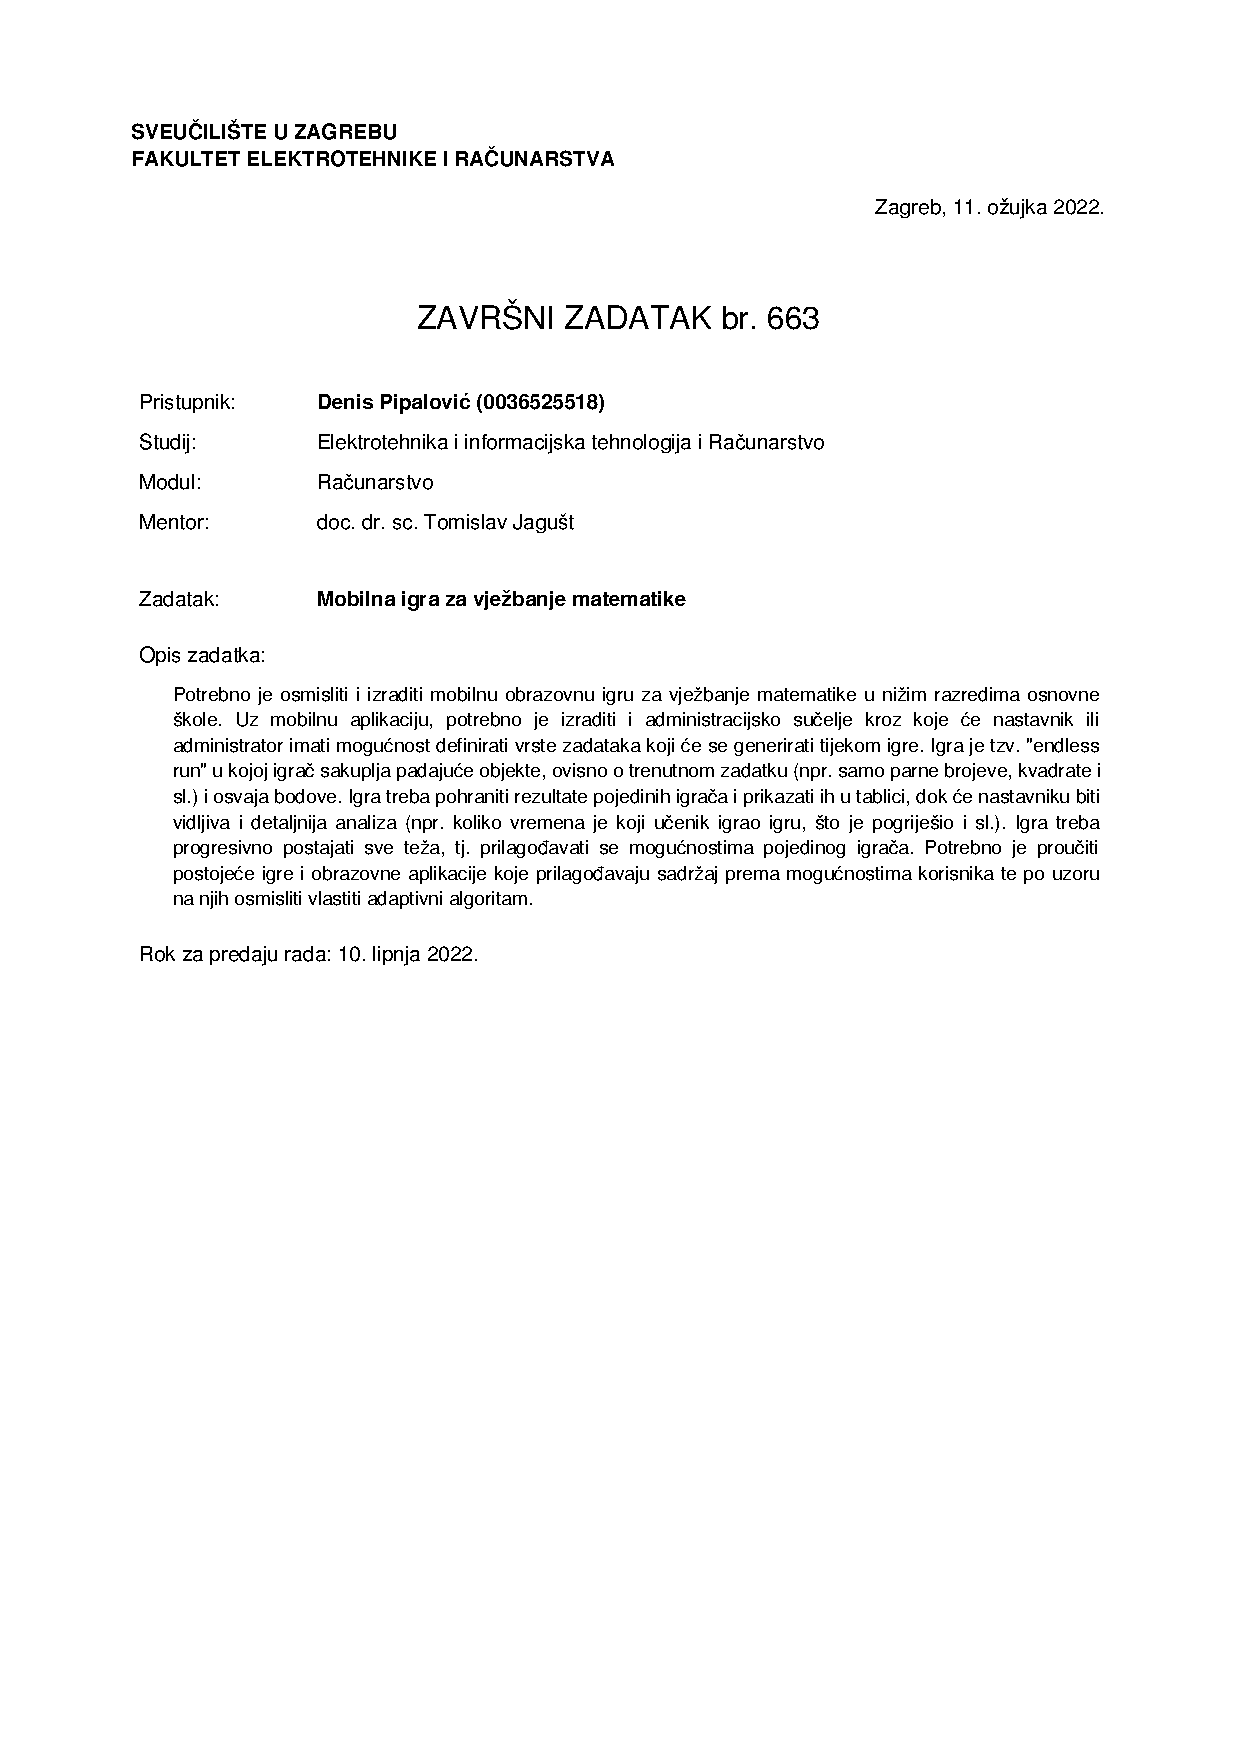
\includepdf[pages={1}]{izvornik.pdf}

% Dodavanje zahvale ili prazne stranice. Ako ne želite dodati zahvalu, naredbu ostavite radi prazne stranice.
\zahvala{}

\tableofcontents

\chapter{Uvod}
	Matematika, osim što je predmet koji se predaje u svim razredima osnovnih i srednjih škola, također je i znanost iz područja prirodnih znanosti.
Značaj matematike vidljiv je ne samo u drugim poljima područja prirodnih znanosti, već i u svim drugim područjima, posebice u području tehničkih znanosti.
Ne poznavanje osnova matematike negativno se odražava na učenikove školske uspjehe kroz cijelo školovanje. Jedan od problema svakako je problem pristupa nastavnika
 u učenju matematike, odnosno manjak povlačenja paralela sa stvarnim svijetom i pokazivanja primjena matematike; ovakav pristup demotivira učenika u vježbanju matematike
i savladavanju čak i osnovnih računskih operacija. Jednom izgubljenu motivaciju za neko područje teško je vratiti nazad.

Primjenom gamifikacije u edukaciji učenicima bi se razne teme i ishodi učenja mogle prezentirati kroz zanimljive načine, samim time i povećati zainteresiranost za nekom temom 
ili predmetom. S obzirom na to da djeca u novije doba koriste pametne uređaje sve više i više, gamifikacija jedan od način kroz koji bi to vrijeme na mobitelu moglo biti potrošeno
 u edukativne svrhe; kroz zabavu!

S obzirom na navedeno, tema ovog rada je napraviti mobilnu igru za vježbanje matematike u nižim razredima osnovne škole koja će kroz zanimljiv i interaktivan način pružati  ugodnije iskustvo
vježbanja matematičkih zadataka. Igra je zamišljena kao tzv. „endless runner“ u kojoj igrač skuplja padajuće objekte ovisno o trenutnom zadatku (npr. samo parne brojeve, brojeve veće od zadanog,
brojeve djeljive s određenim brojem, samo kvadrate i slično) i sakuplja bodove. Kako igra ne bi postala monotona kroz kratko vrijeme igranja cilj je napraviti da igra postaje progresivno sve teža
i teža, no do te mjere da se ne postigne negativan efekt u drugom ekstremu; igra ne smije postati niti previše teška jer bi samim time postala i demotivirajuća! Stoga je cilj da se težina igre
dinamički prilagođava mogućnostima učenika. Osim same mobilne igre, potrebno je izgraditi i jednostavno web sučelje za učitelja kako bi mogao postavljati tipove zadataka koji prate temu onoga što
se trenutno predaje na nastavi. Kroz navedeno web sučelje nastavniku će se pružati i mogućnost pregleda rezultata pojedinog učenika te uvid u detalje igre kao što je tip zadatak na kojem je učenik 
griješio, ukupno vrijeme igranja i slično. Kako bi igra bila dostupna svima koji ju požele igrati, odnosno kako igra ne bi ovisila o postavkama učitelja, postojati će i zadane postavke koje će se moći
 prilagođavati kroz postavke same igre. 



\chapter{Cilj projekta}
Cilj projekta je izrada mobilne igre za vježbanje matematike popraćene web stranicom koja služi za zadavanje zadataka i pregled rezultata igre. Cilj mobilne igre napraviti je vježbu matematike zanimljiviju učenicima, 
dok je cilj web stranice učiteljima olakšati zadavanje zadataka, praćenje i pohranu rezultata učenika na jednostavniji način.

	\section{Mobilna igra}
	Mobilna igra većinski je dio projekta. Kroz ovu igru učenici nižih razreda na zanimljiviji način mogu vježbati određeno gradivo matematike. Igra osim što se može igrati s predefiniram postavkama zadataka također omogućava uređivanje istih
	te preuzimanje postavki koje su napravljene preko web sučelja za učitelja. Ukoliko učenik igra igru sa preuzetim postavkama napravljenim preko web sučelja, podaci o njegovoj igri bit će dostavljeni učitelju po završetku igre.
	Iz glavnog menija igre možemo pristupiti glavnom ekranu igre i postavkama.
		
		\subsection{Glavni ekran igre}
		Na glavnom ekranu igre nalazi se sav takoreći učenicima zanimljiv sadržaj, odnosno mjesto gdje se sama igra i igra. Igra je "endless runner" i tematski je zamišljena kao put iz središta zemlje ka dubokom svemiru, odnosno to je ono što pokazuje
		pozadina koja putuje prema dolje, što stvara efekt putovanja objekta koji se upravlja prema gore. Objekt koji je upravljan moguće je pomicati lijevo-desno i tako skupljati padajuće objekte koje je potrebno skupiti ovisno o trenutnom zadatku,
		odnosno izbjegavati one koji krše pravila trenutnog zadatka. Padajući objekti konstanto se stvaraju i njihov sadržaj ovisi o tome koji je trenutni zadatak ili koja je trenutna težina igre. Odnosno svaki zadatak osim što ima svoj opis ima i određene
		parametre, tako bi recimo zadak "skupljaj brojeve veće ili jednake 18", osim navedenog opisa, relativnog broja 18 imao i definirane parametre kao što je minimalna i maksimalna granica iz kojeg seta se brojevi mogu dodjeliti; nadalje, pri većoj 
		težini igre se na padajućem objektu možda neće prikazati broj direktno, već u obliku matematičke operacije, npr. "29 - 12".
		\begin{figure}[H]
			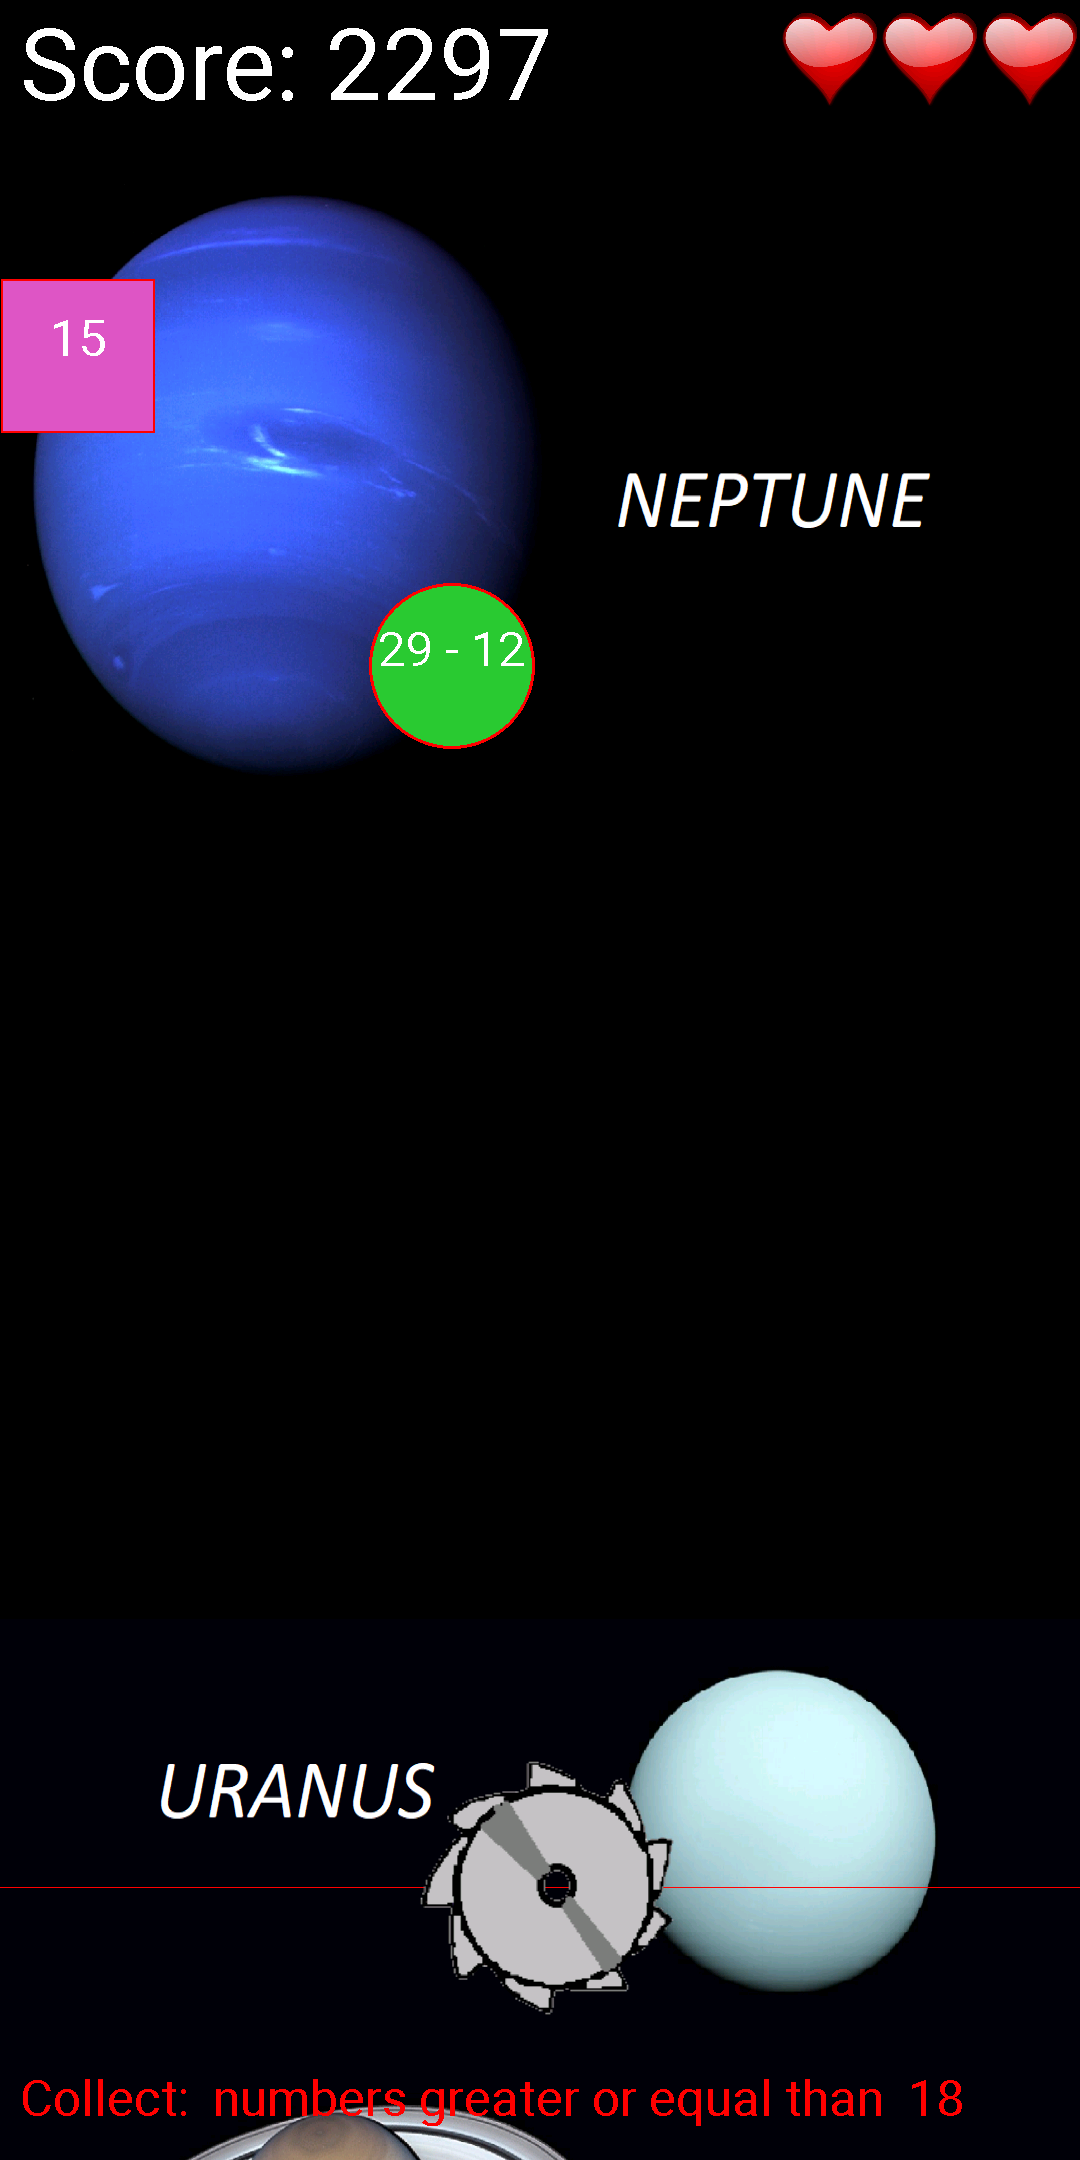
\includegraphics[scale = 0.225]{"slike/igra.png"} 
			\centering
			\caption{Ideja igre}
			\label{fig:idejaigre}
		\end{figure}
		
		Igranjem igre i sakupljanjem objekata koji odgovaraju trenutačnom zadatku učenici skupljaju bodove; te je cilj po završetku igre imati što veći broj bodova. Završetak igre odgovara gubitku tri života.
		Bodovanje na primjeru  za zadatak "skupljaj parne brojeve" :
		\begin{itemize}
				\item  {Igrač je pokupio paran broj : +100 bodova}
				\item  {Igrač NIJE pokupio paran broj: -100 bodova}
				\item  {Igrač je pokupio neparan broj: Gubitak života}
		\end{itemize}
		
		S obzirom da se može dogoditi situacija u kojoj se preklapaju dva objekta, odnosno situacija u kojoj se preklapaju objekt koji se ne smije pokupiti i objek koji se mora pokupiti (u ovom slučaju parni i neparni broj); kako se igrač ne bi osjećao
		zakinutim nakon gubitka 100 bodova zbog objekta kojeg je morao propustiti kako ne bi izgubio jedan život, igrač je za svakih 10 osvježavanja ekrana nagrađen sa jednim bodom. U konačnici ispada da igrač smije propustiti jedan objekt svakih 15 do 20 sekundi
		kako bi se poništili bonus bodovi sa izgubljenim bodovima za ne skupljanje odgovarajućeg objekta. Preklapanje dva objekta se ne događa toliko često stoga igrač samim trajenjem igre skuplja dodatne bodove.
		\newline
		Trenutačni broj bodova prikazan je na vrhu zaslona sa lijeve strane, dok je na desnoj strani prikazan broj života koji odgovara broju sličica srca. Na donjem dijelu ekrana moguće je vidjeti trenutačni zadatak.
		Svaki zadatak traje od prilike pola minute, a promijena zadatka odvija se na način da prvo prestanu padati novi objekti. Kada više nema padajućih objekata na ekranu, slučajnim odabirom se bira sljedeći zadatak te se tekst novog zadatka
		pokazuje kako u donjem dijelu ekrana tako i na samoj sredini ekrana na nekoliko sekundi kako bi igrač bio u potpunosti svjestan promjene zadatka. 

		
		\subsection{Predefinirane postavke}
		Kako igra ne bi ovisila isključivo o postavkama koje zadaje učitelj, odnosno kako bi se mogla igrati neposredno nakon instalacije, osmišljene su predefinirane postavke koje sadrže zadatke prilagođene ponajviše prvom razredu osnovne škole.
		Neki od predefiniranih zadataka su: 
			\begin{itemize}
				\item  {Skupljaj parne brojeve}
				\item  {Skupljaj neparne brojeve}
				\item  {Skupljaj brojeve veće od \textit{x}}
				\item  {Skupljaj brojeve manje od \textit{x}}
				\item  {Skupljaj brojeve veće ili jednake \textit{x} koji su parni }
				\item  {Skupljaj kvadrate}
				\item  {Skupljaj kružnice}
				\item {i slično}
			\end{itemize}
		Osim što igra omogućava ove i druge predefinirane postavke, također omogućava i njihovo uređivanje, odnosno njihovo uključivanje te isključivanje; kako bi si učenici samostalno mogli prilagoditi zadatke na koje žele staviti naglasak dok vježbaju.
		Svako uključivanje, odnosno isključivanje navedenog zadatka ostaje zapamćeno i koristi se pri pokretanju igre.
		
		\begin{figure}[H]
			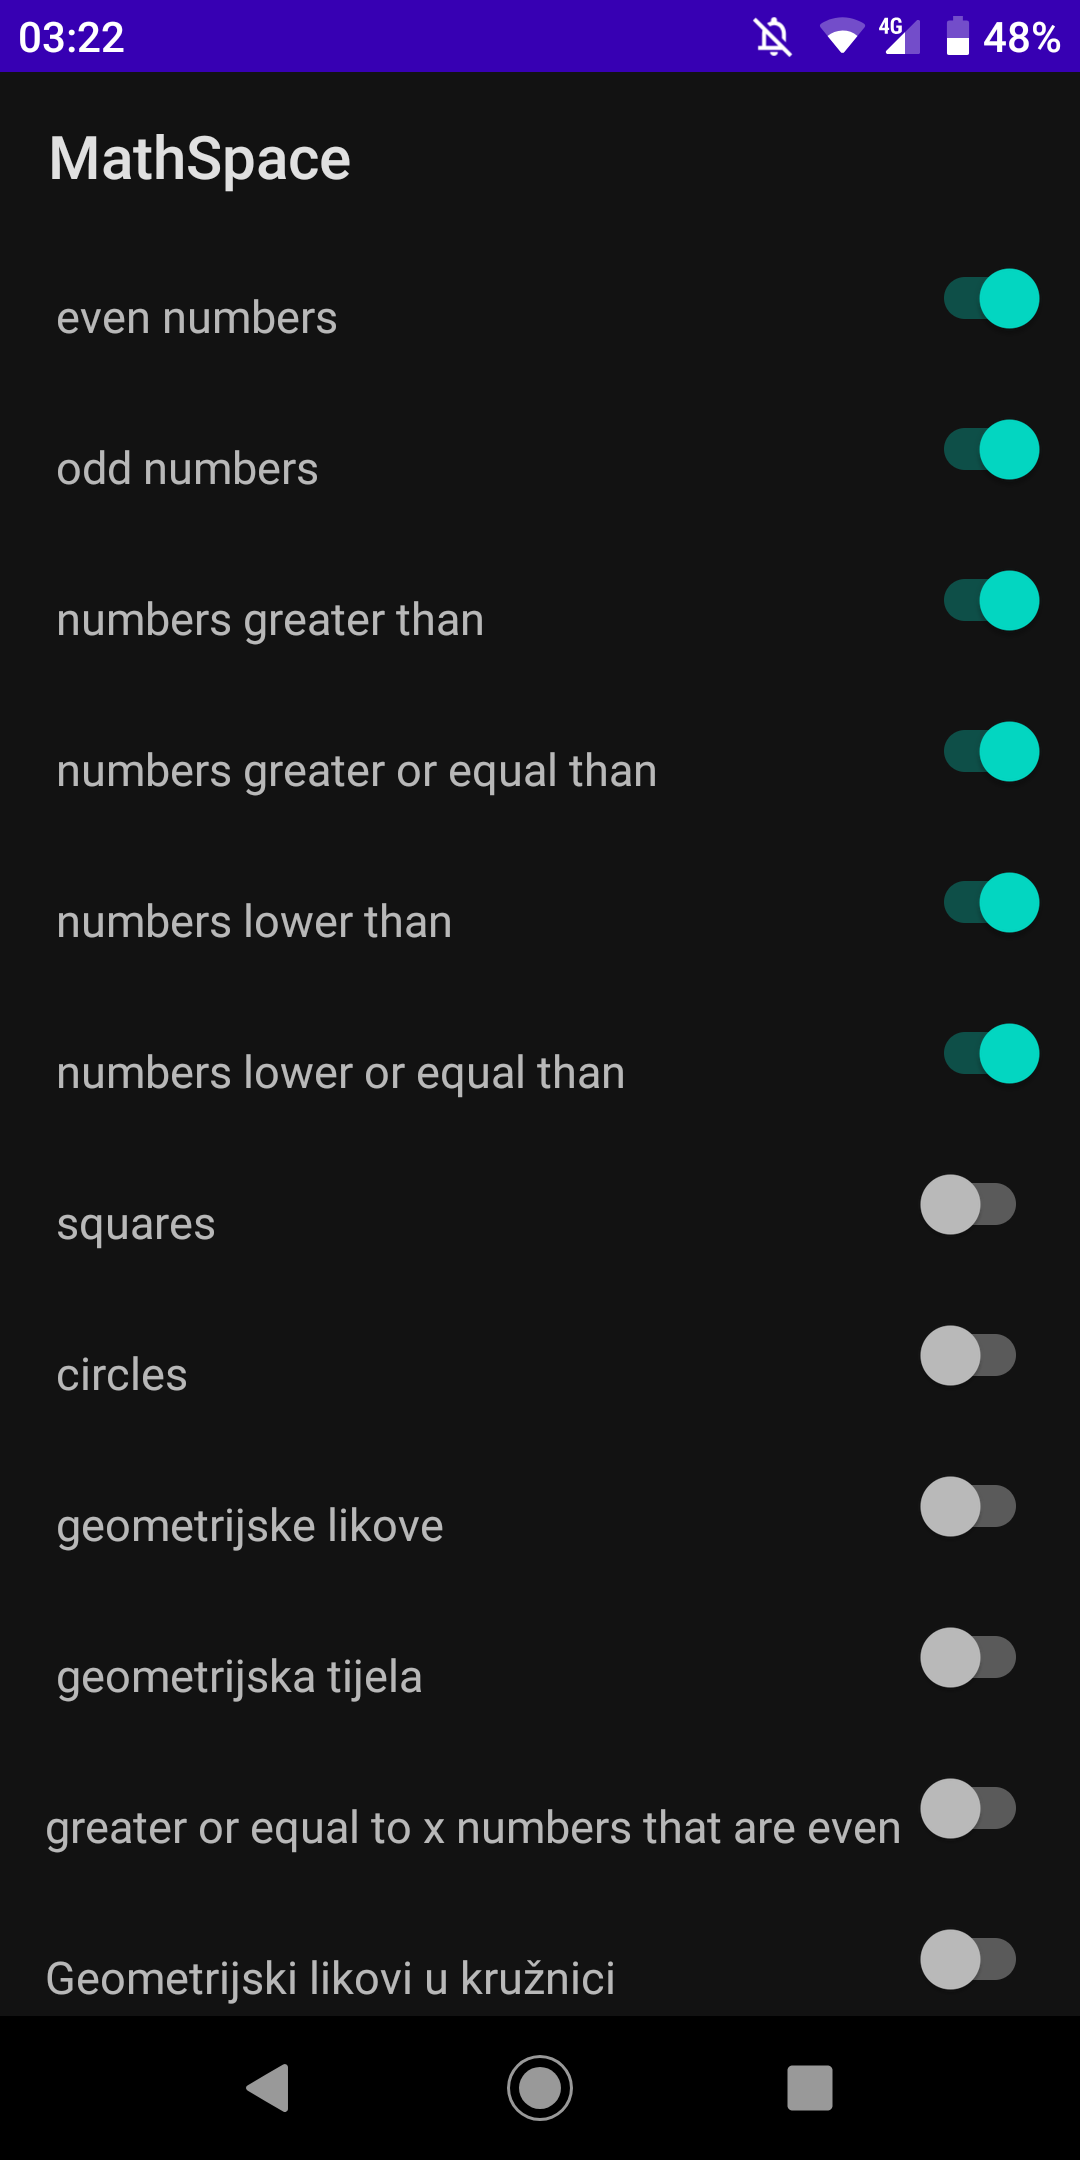
\includegraphics[scale = 0.1]{"slike/defaulttasks.png"} 
			\centering
			\caption{Ideja Uključivanje/isključivanje predefiniranih postavki}
			\label{fig:idejaigre}
		\end{figure}
		

		\subsection{Preuzete postavke}
		Osim predefiniranih postavki igra nudi mogućnost preuzimanja postakvi izrađenih preko web stranice. Kako bi igrač mogao preuzeti postavke prvo treba postaviti korisničko ime te nakon toga u za to previđeno polje upisati identifikator postavki
		koje želi preuzeti i za kraj pritisnuti tipku za preuzimanje postavki. 
	
		\begin{figure}[H]
			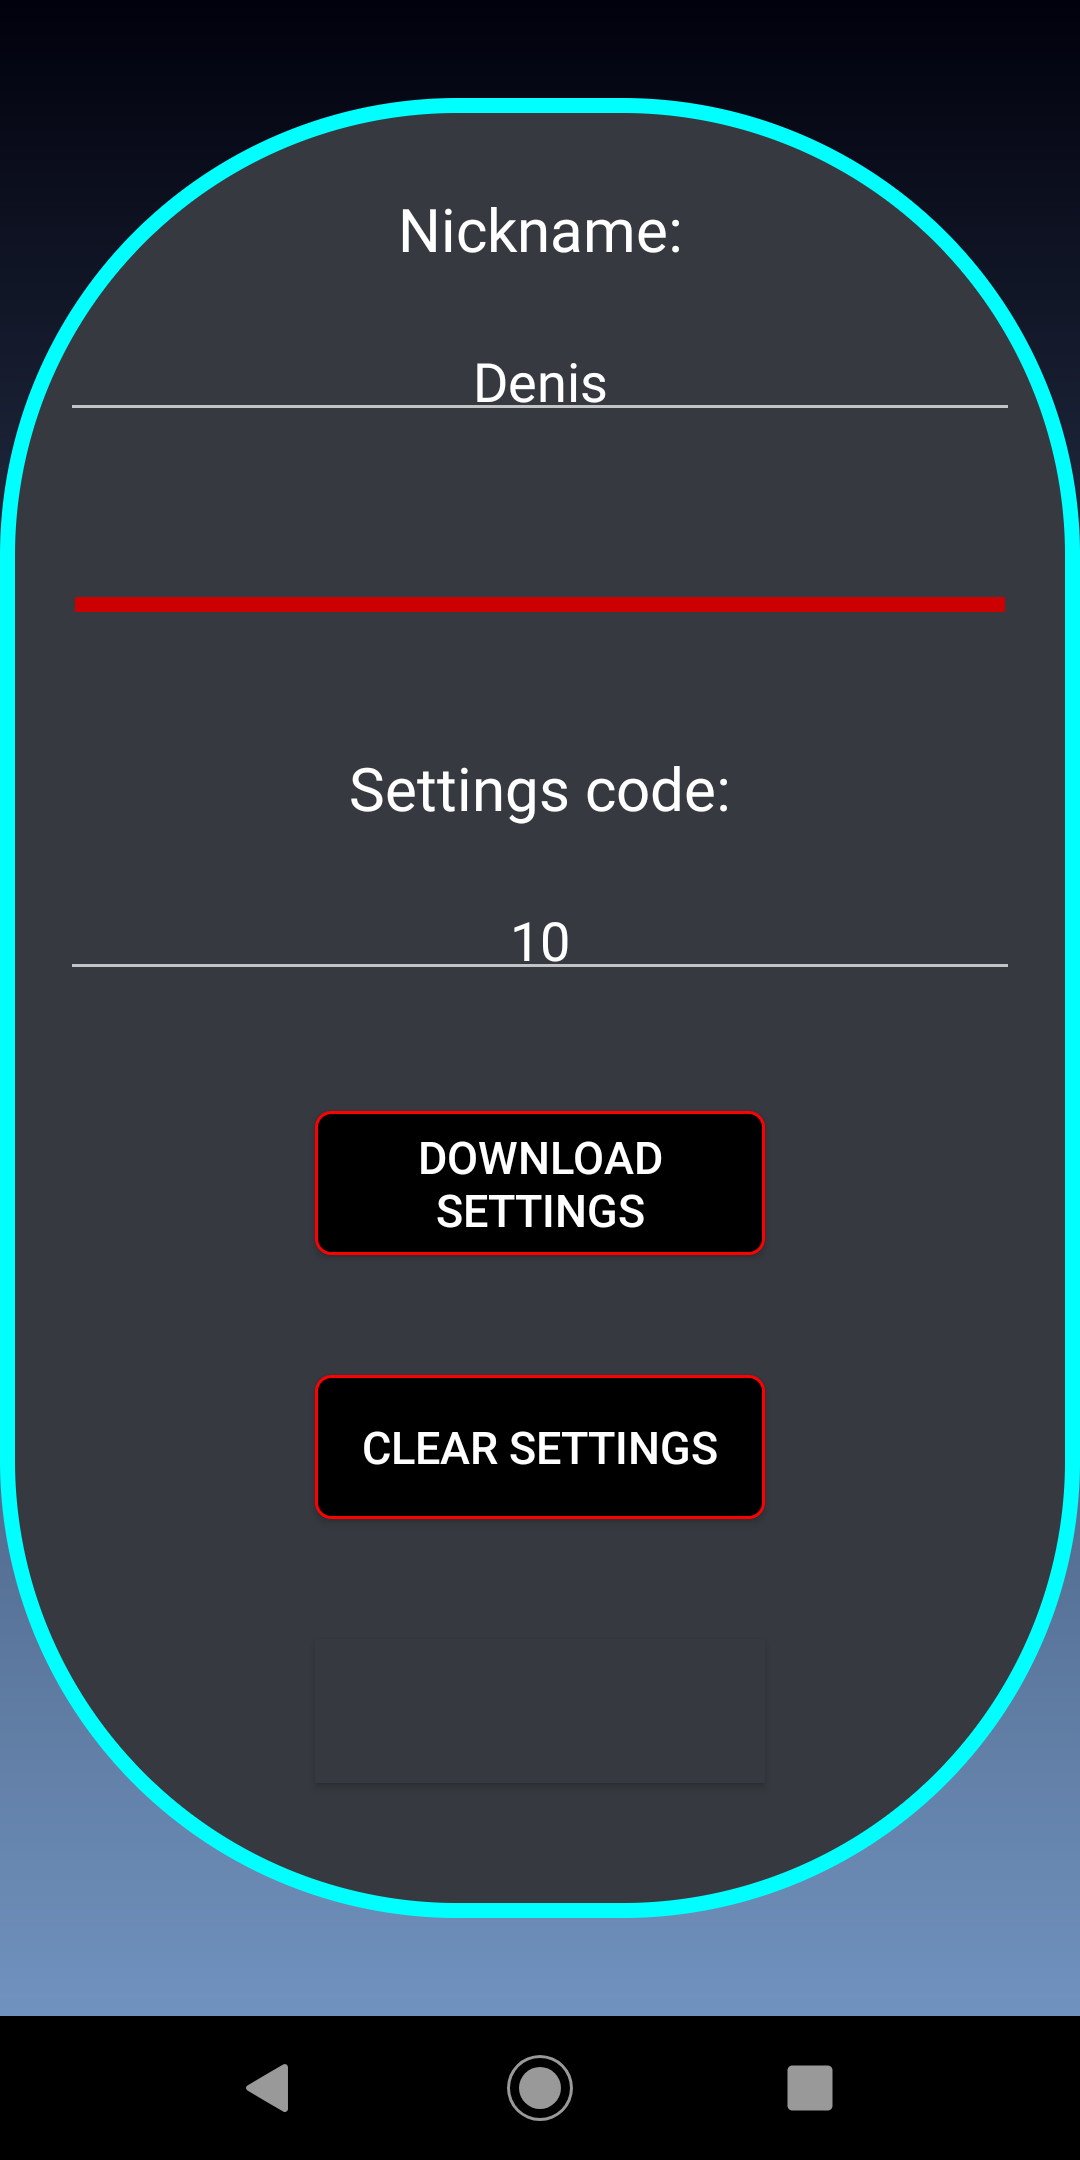
\includegraphics[scale = 0.2]{"slike/downloadsettings.png"} 
			\centering
			\caption{Preuzimanje postavki s interneta}
			\label{fig:preuzimanjepostavki}
		\end{figure}
		
		Jednom kad je igrač preuzeo postavke s interneta sada mu se na izbor u glavnom meniju postavki pruža mogućnost odabira koje postavke želi koristiti; one preuzete s interneta ili one predefinirane!
		
				\begin{figure}[!htb]
			\begin{minipage}{0.48\textwidth}
				\centering
				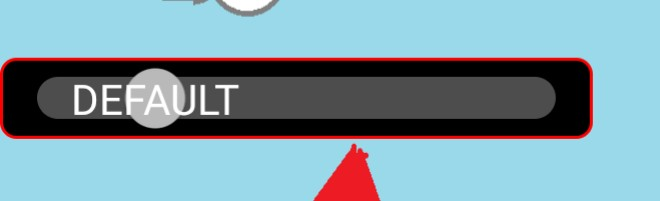
\includegraphics[scale=0.25]{"slike/usedefault.jpg"} 
				\caption{Odabir korištenja predefiniranih postavki}
				\label{fig:saw1}
			\end{minipage}\hfill
			\begin{minipage}{0.48\textwidth}
				\centering
				
\includegraphics[scale=0.25]{"slike/usedownloaded.jpg"} 
				\caption{Odabir korištenja preuzetih postavki}
				\label{fig:saw2}
			\end{minipage}
		\end{figure}
		
		

	\section{Web stranica}
	Web stranica drugi je dio projekta, ujedno i manji. Kroz ovu web stranicu učiteljima se na jednostavan način omogućava izrada zadataka, odnosno postavljanje pravila na osnovu kojih će se zadaci automatski generirati.
	Osim zadavanja zadataka stranica nudi i mogućnost pregleda rezultata pojedinih učenika i dodatne dalje svakog igranja. Za mogućnost izrade postavki, stoga i pregled rezultata igrara korisnik se mora prvo prijaviti u sustav, odnosno
	registrirati ukoliko nema korisnički račun.

	\subsection{Izrada postavki}
	Izrada postavki generalno je jednostavan i izravan (engl. \textit{straightforward}) proces. Nakon logiranja u sustav korisniku se nudi opcija "\textit{My Games}" na izbornoj traci. Odabirom ove stavke korisniku se prikazuju sve
	njegove postojeće grupe postavke igara i mogućnost izrada nove grupe postavki. 
	
		\begin{figure}[H]
			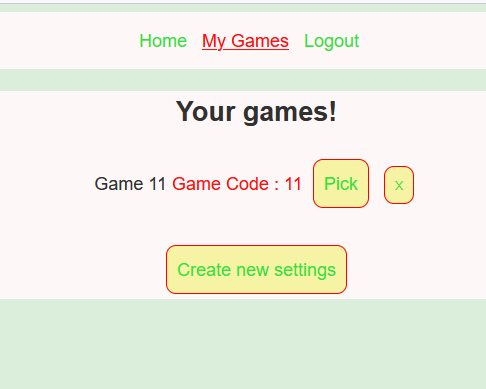
\includegraphics[scale = 0.7]{"slike/izradapostavki.png"} 
			\centering
			\caption{My Games}
			\label{fig:izradapostavki}
		\end{figure}
	
	Odabir postojeće grupe postavki moguće je učiniti pritiskom na gumb "\textit{Pick}" uz postavke koje želimo odabrati, odnosno ukloniti grupu postavki klikom na  gumb "\textit{X}". Izrada nove grupe postavki može se napraviti klikom na gumb
	 "\textit{Create new settings}". 
	 

	 Nakon odabira određene grupe postavki korisniku se nudi mogućnost pregleda do sad napravljenih postavki pa tako i dodavanja nove postavki u odabranu grupu. Kako bi korisnik dodao novu postavku u grupu postavki prvo se treba odlučiti koji 
	 tip postavke želi dodati. 
	 	\begin{figure}[H]
			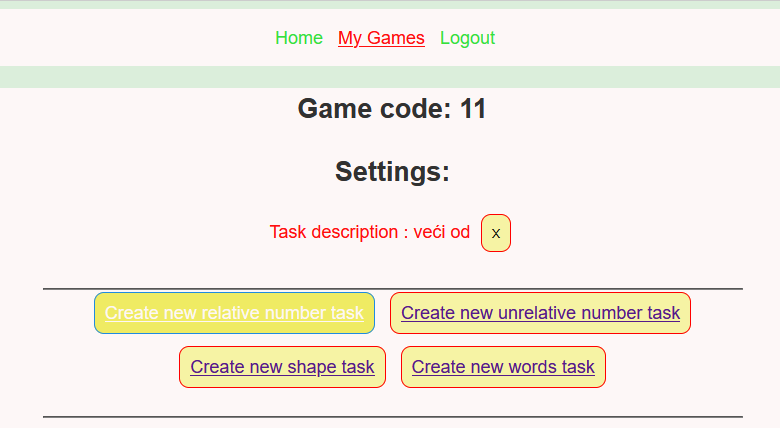
\includegraphics[scale = 0.7]{"slike/zadavanjepostavki.png"} 
			\centering
			\caption{Pregled i izrada postavki unutar neke grupe postavki}
			\label{fig:pregledpostavki}
		\end{figure}
	Na primjer, ukoliko korisnik želi zadati postavku koja od igrača mobilne igre traži da skuplja brojeve djeljive sa tri, potrebno je pritisnuti \textit{Create new relative number task} nakon čega se prikazuje novi ekran koji to omogućava.
	\begin{figure}[H]
		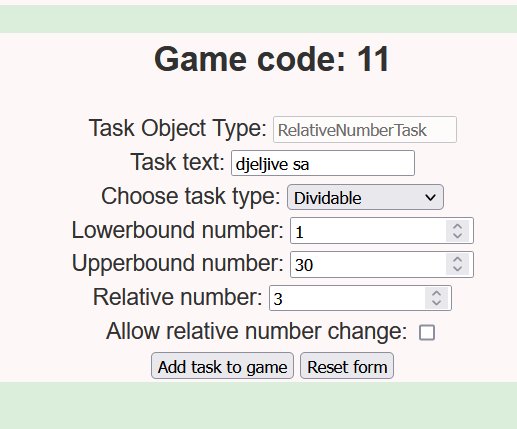
\includegraphics[scale = 0.9]{"slike/zadavanjekonkretnepostavke.png"} 
		\centering
		\caption{Izrada konkretne postavke}
		\label{fig:izradapostavkedjeljenje}
	\end{figure}
		
		Web stranica od korisnika traži unos teksta koji će opisivati zadatak, odabir tipa zadatka, donju i gornju granicu iz koje će se generirati brojevi na padajućim objektima, relativan broj odnosno, s obzirom da želimo zadati da je zadatak
		skupljati brojeve djeljive sa 3 - to je u ovom slučaju broj 3! Za kraj nudi se opcija promjene relativnog broja po završetku zadatka (novi broj slučajno bi se odredio iz skupa [lowerbound number, upperbound number]), što u ovom slučaju ne bismo
		htjeli. Ova opcija najviše je pogodna za zadatke koji od korisnika traže da skupljaju brojeve veće/manje od relativnog broja. Za završetak izrade postavke potrebno je odabrati \textit{Add task to game}.
	
	\subsection{Pregled rezultata}
	Nakon igranja igre na mobilnoj igri s preuzetim postavkama rezultati igre i njeni detalji postaju vidljivi korisniku web stranice koji je napravio korištene postavke. 
	Površni pregled koji prikazuje zapise o igrama prikazuje samo ime igrača, vrijeme prihvata podataka i konačni rezultat.
	\begin{figure}[H]
		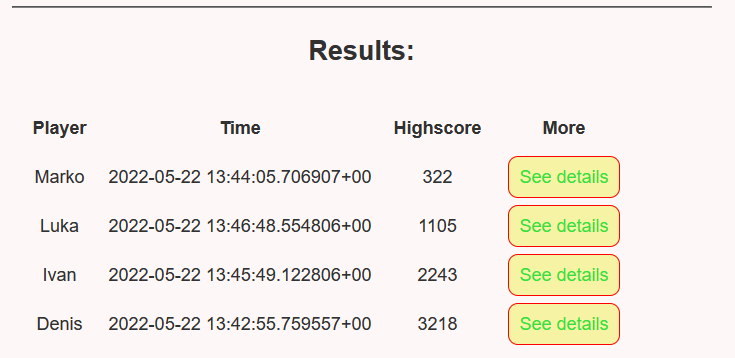
\includegraphics[scale = 0.9]{"slike/pregledsvihrezultata.png"} 
		\centering
		\caption{Pregled svih rezultata}
		\label{fig:pregledsvihrezultata}
	\end{figure}
	
	Odabirom gumba \textit{See details} korisniku web stranice pruža se mogućnost pregleda više detalja, odnosno mogućnost pregleda detalja cijelog tijek igre. Konkretnije omogućen je uvid u svaki značajniji događaj i njegovo vrijeme.
	Značajniji događaji su:
		\begin{itemize}
				\item  {Promjena zadatka - prikazano crnom bojom}
				\item  {Skupljen odgovarajući padajući objekt (+100 bodova) - prikazano zelenom bojom}
				\item  {Nije skupljen odgovarajući padajući objekt (-100 bodova) - prikazano naračastom bojom}
				\item  {Skupljen neodgovarajući objekt (izgubljen život) - prikazano crvenom bojom}
		\end{itemize}
	Radi jednostavnosti pregleda događaja igre, određeni događaji su istaknuti određenom bojom.
	
	\begin{figure}[H]
		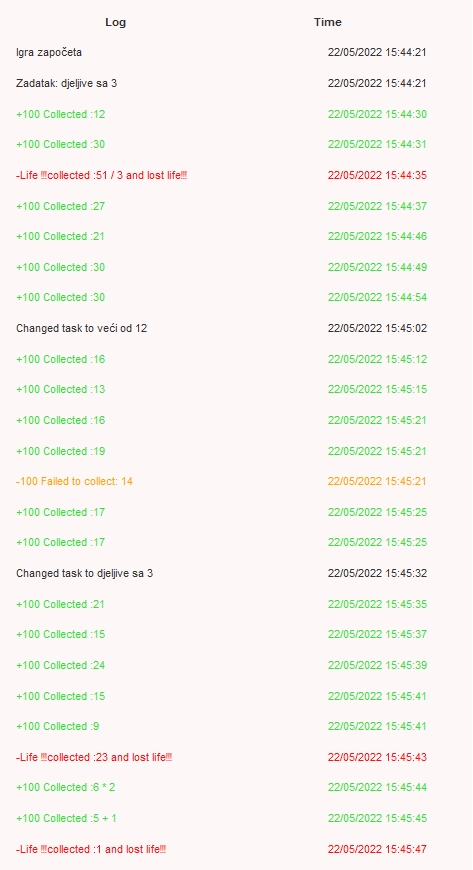
\includegraphics[scale = 0.9]{"slike/detaljanpregledrezultata.png"} 
		\centering
		\caption{Detaljan pregled jedne igre}
		\label{fig:pregledjedneigre}
	\end{figure}
	

\chapter{Usporedba sa sličnim igrama}
Postoje mnogobrojne Android igre dostupne na Google Play marketu koje kao su prikazane kao igre koje služe u edukativne svrhe, odnosno specifično kao igre za vježbanje matematike.  U nastavku je usporedba igre koja je tema ovog rada sa naizgled 
sličnim postojećim igrama; uz to valja i napomenuti da je po slobonoj procijeni više od 90 posto matematičkih igara bazirano na tipu kviza sa 4 ponuđena odgovora. Prednost igre koja je tema ovog rada nad navedenim igrama je mogućnost pregleda tijeka događaja.
	
	\section{Toon Math Runner} 
	"\textit{Toon Math Runner}" (u nastavku TMR) je vizualno lijepa 2.5D mobilna igra za vježbanje matematike. Ova igra nudi opciju otključavanja raznih karaktera u zamijenu za novčiće koje igrač može skupljati. Igrač upravlja karakterom
		na način da upravljenog karaktera može pozicionirati u jednoj od tri linije, osim toga nudi se mogućnost skakanja i saginjanja. Ova igrica uvelike podsjeća na popularnu igricu "\textit{Subway Surfers}" kako po načinu igranja, tako i vizualno.
	 Nažalost, TMR nije tkz. "endless runner" uz to što niti vježbanje matematike nije u glavnom fokusu. Glavni fokus igre je sakupljanje novčića uz pojavljivanje jednog matematičkog zadatka u prosjeku jednom u pola minute. Osim što se ova igra 
	 pokušava nazvati igrom za vježbanje matematike, valja naglasiti da je velika zastupljenost reklama u istoj. \begin{figure}[!htb]
		\begin{minipage}{0.48\textwidth}
			\centering
			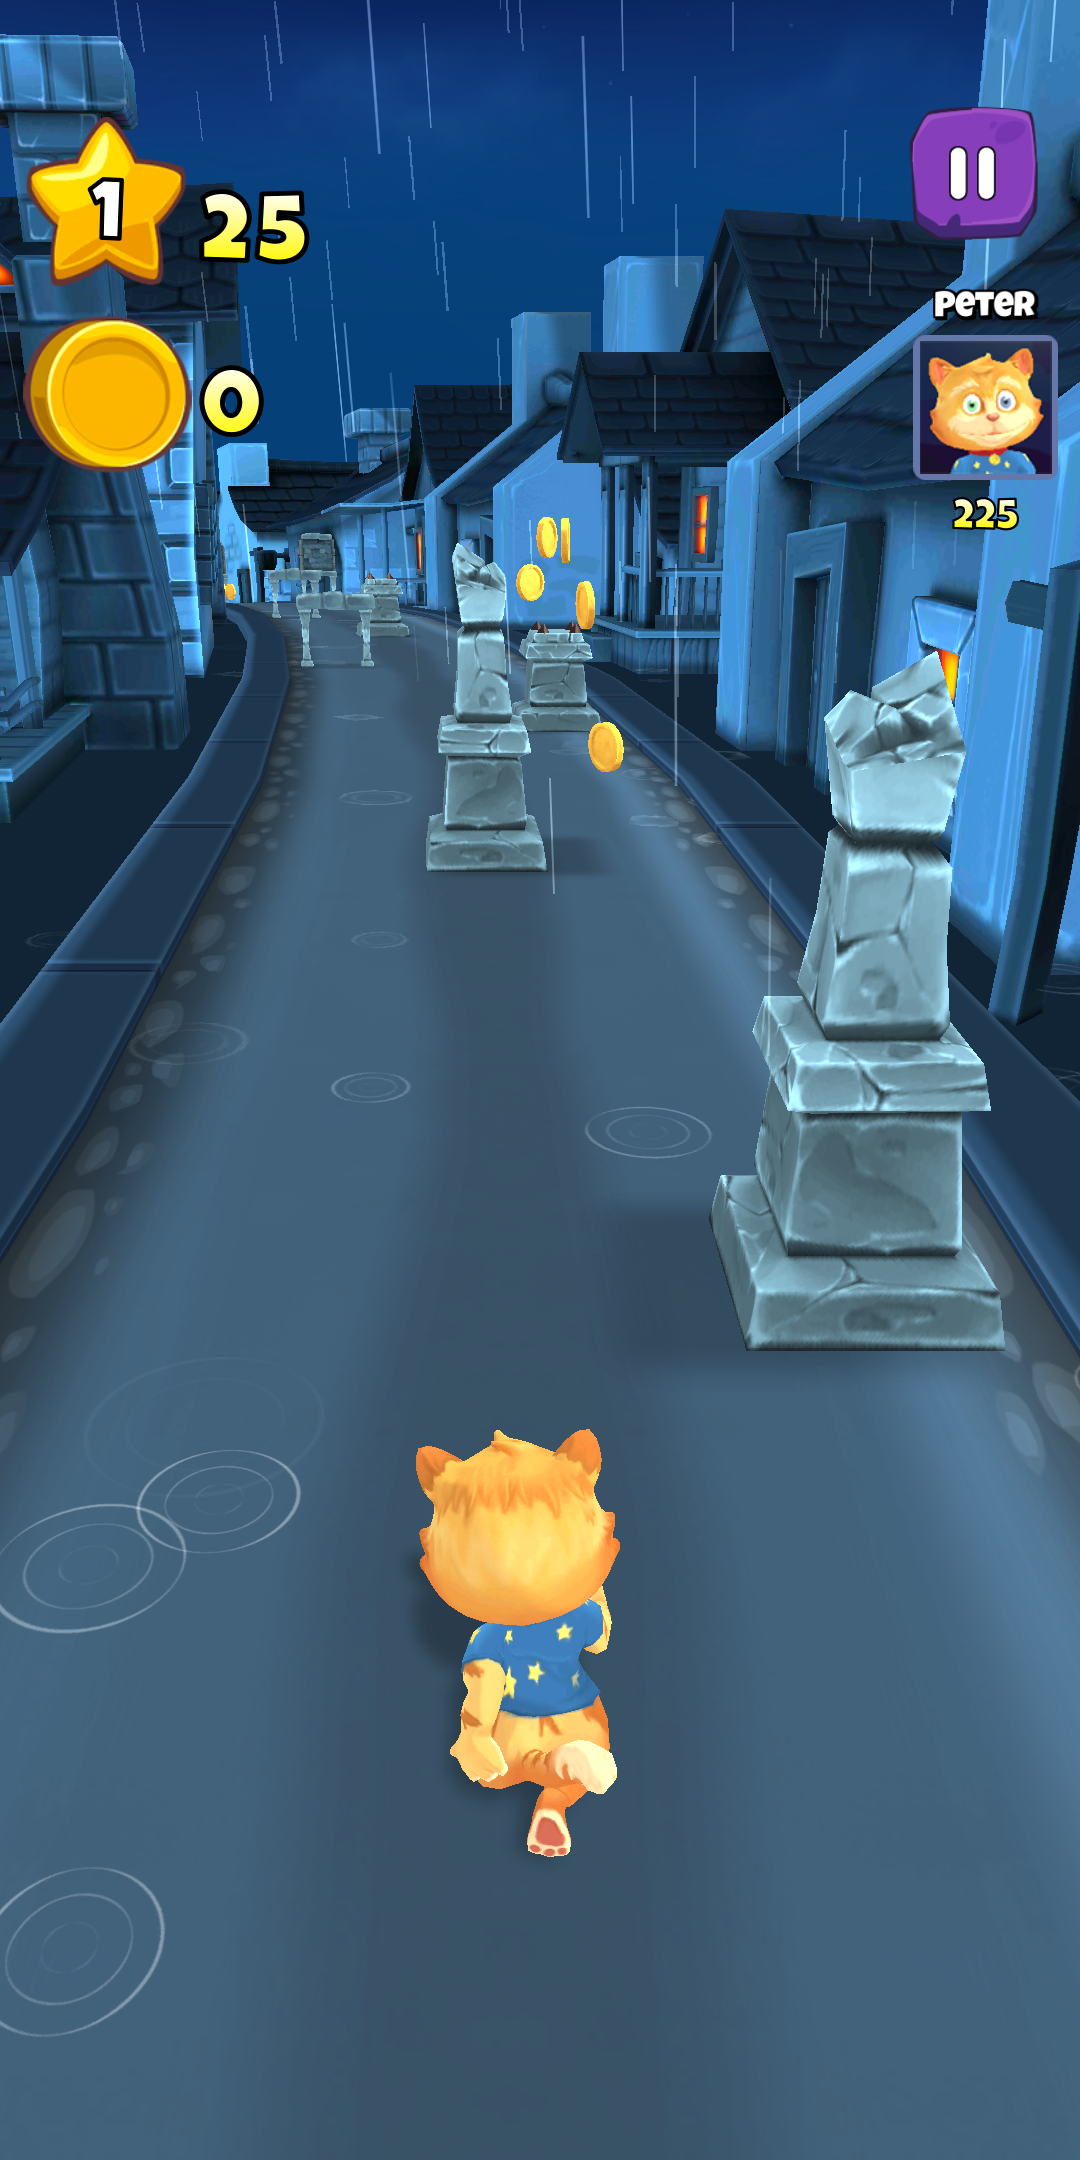
\includegraphics[scale=0.15]{"slike/igre/toonmath1.png"} 
			\caption{Većina igre - skupljanje novčića}
			\label{fig:skupljewnjenovcica}
		\end{minipage}\hfill
		\begin{minipage}{0.48\textwidth}
			\centering
			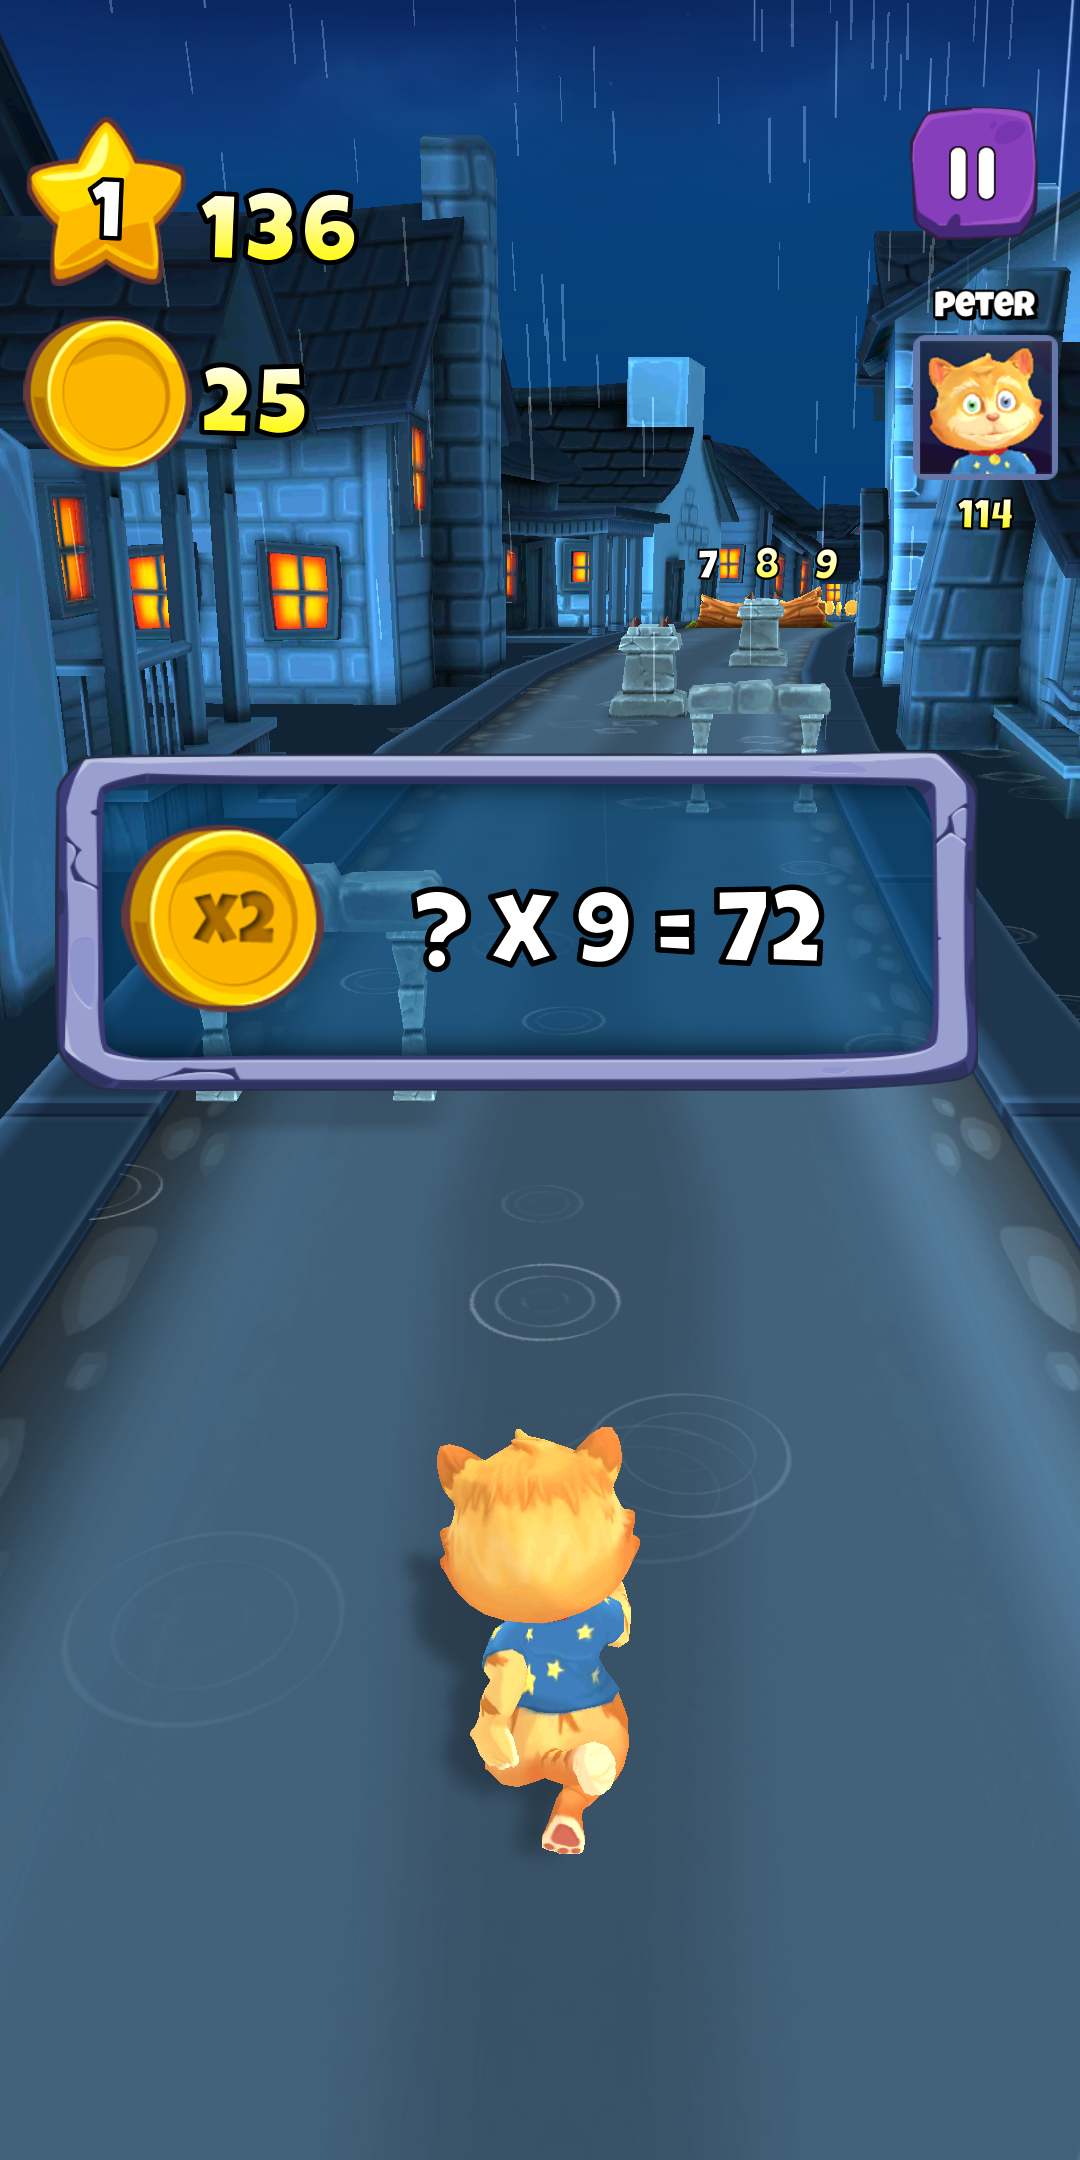
\includegraphics[scale=0.15]{"slike/igre/toonmath2.png"} 
			\caption{Matematički zadatak}
			\label{fig:toonmathmath}
		\end{minipage}
	\end{figure}
 
	 Prednost ove igre u odnosu na igru ovog rada je svakako vizualni izgled i mogućnost napretka u vidu otključavanja drugih karaktera, dok je nedostatak manjak matematičkih zadataka te količina reklama. 
		

	
	\section{Math jumps: Math Games}
	"\textit{Math jumps: Math Games}" (u nastavku MJMG) je vizualno lijepa 2.5D mobilna igrica za vježbanje matematike. Ova igrica osim što je vizualno ugodna, osmišljena je na zanimljiv način. Igrač koji igra igricu predstavljen je kao karakter
	u vagonu koji se vozi po tračnicama. Ovim karakterom ne upravlja se izravno već se njegovo postupanje odvija u skladu s time da li je igrač točno odgovorio na postavljeno matematičko pitanje. Npr. ukoliko igrača ispravno odgovori na zadano matematičko
	pitanje, vagon će poskočiti, odnosno skrenuti kada za tim ima potrebu, suprotno vagon će samo nastaviti voziti ravno i odletiti u provaliju, u tom slučaju igrač gubi život. Igrica je tkz. "endless runner" i moguće je podešavati računske operacije
	koje se mogu pojaviti u zadacima. Ova igra također nudi otključavanje raznih "skinova".
	
	\begin{figure}[H]
		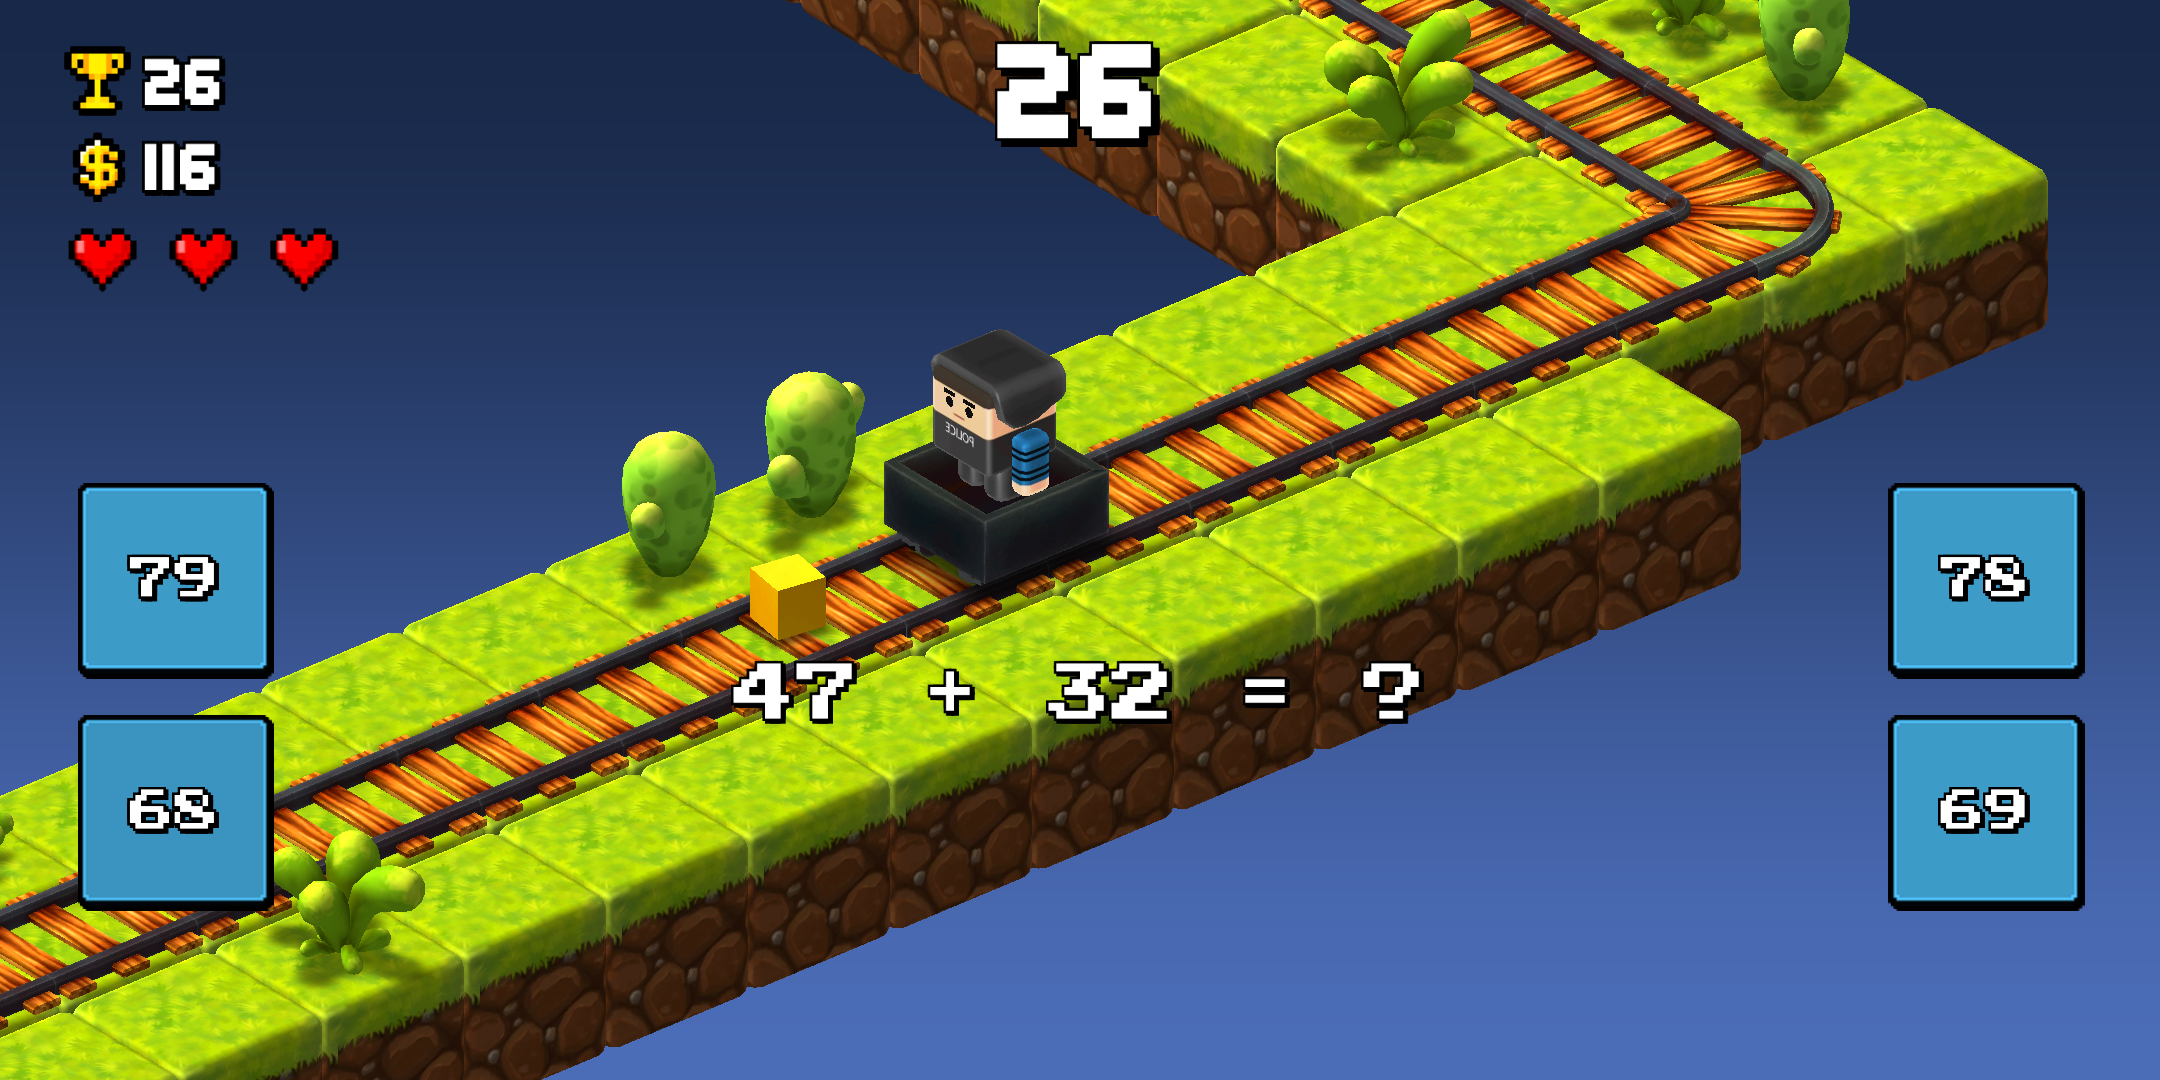
\includegraphics[scale = 0.2]{"slike/igre/mathjumps.png"} 
		\centering
		\caption{Primjer zadatka igre MJMG}
		\label{fig:mjmg}
	\end{figure}
	
	MJMG je u večini aspekata bolja igrica od igrice koja je tema ovog rada no moglo bi se reći da je nedostatak MJMG taj da se sva interakcija odvija putem 4 gumba za odgovore, generalno igrica je običan kviz.
	
	
	\section{Mathematical Run (Math games)}
	"\textit{Mathematical Run (Math games)}" (u nastavku MRMG) je 2D mobila igrica za vježbanje matematike. Igrač koji igra igru upravlja sa malom točkicom koja se može nalaziti u jednoj od tri trake. Na ekranu se prvobitno pojavljuje zadatak, a potom 3
	ponuđena odgovora. Kako bi igrač pokupio ispravan odgovor, treba se pozicionirati u za to odgovarajuću traku. Same kontrole upravljanja su dosta loše, dosta često neresponzivne.
	
			\begin{figure}[!htb]
			\begin{minipage}{0.48\textwidth}
				\centering
				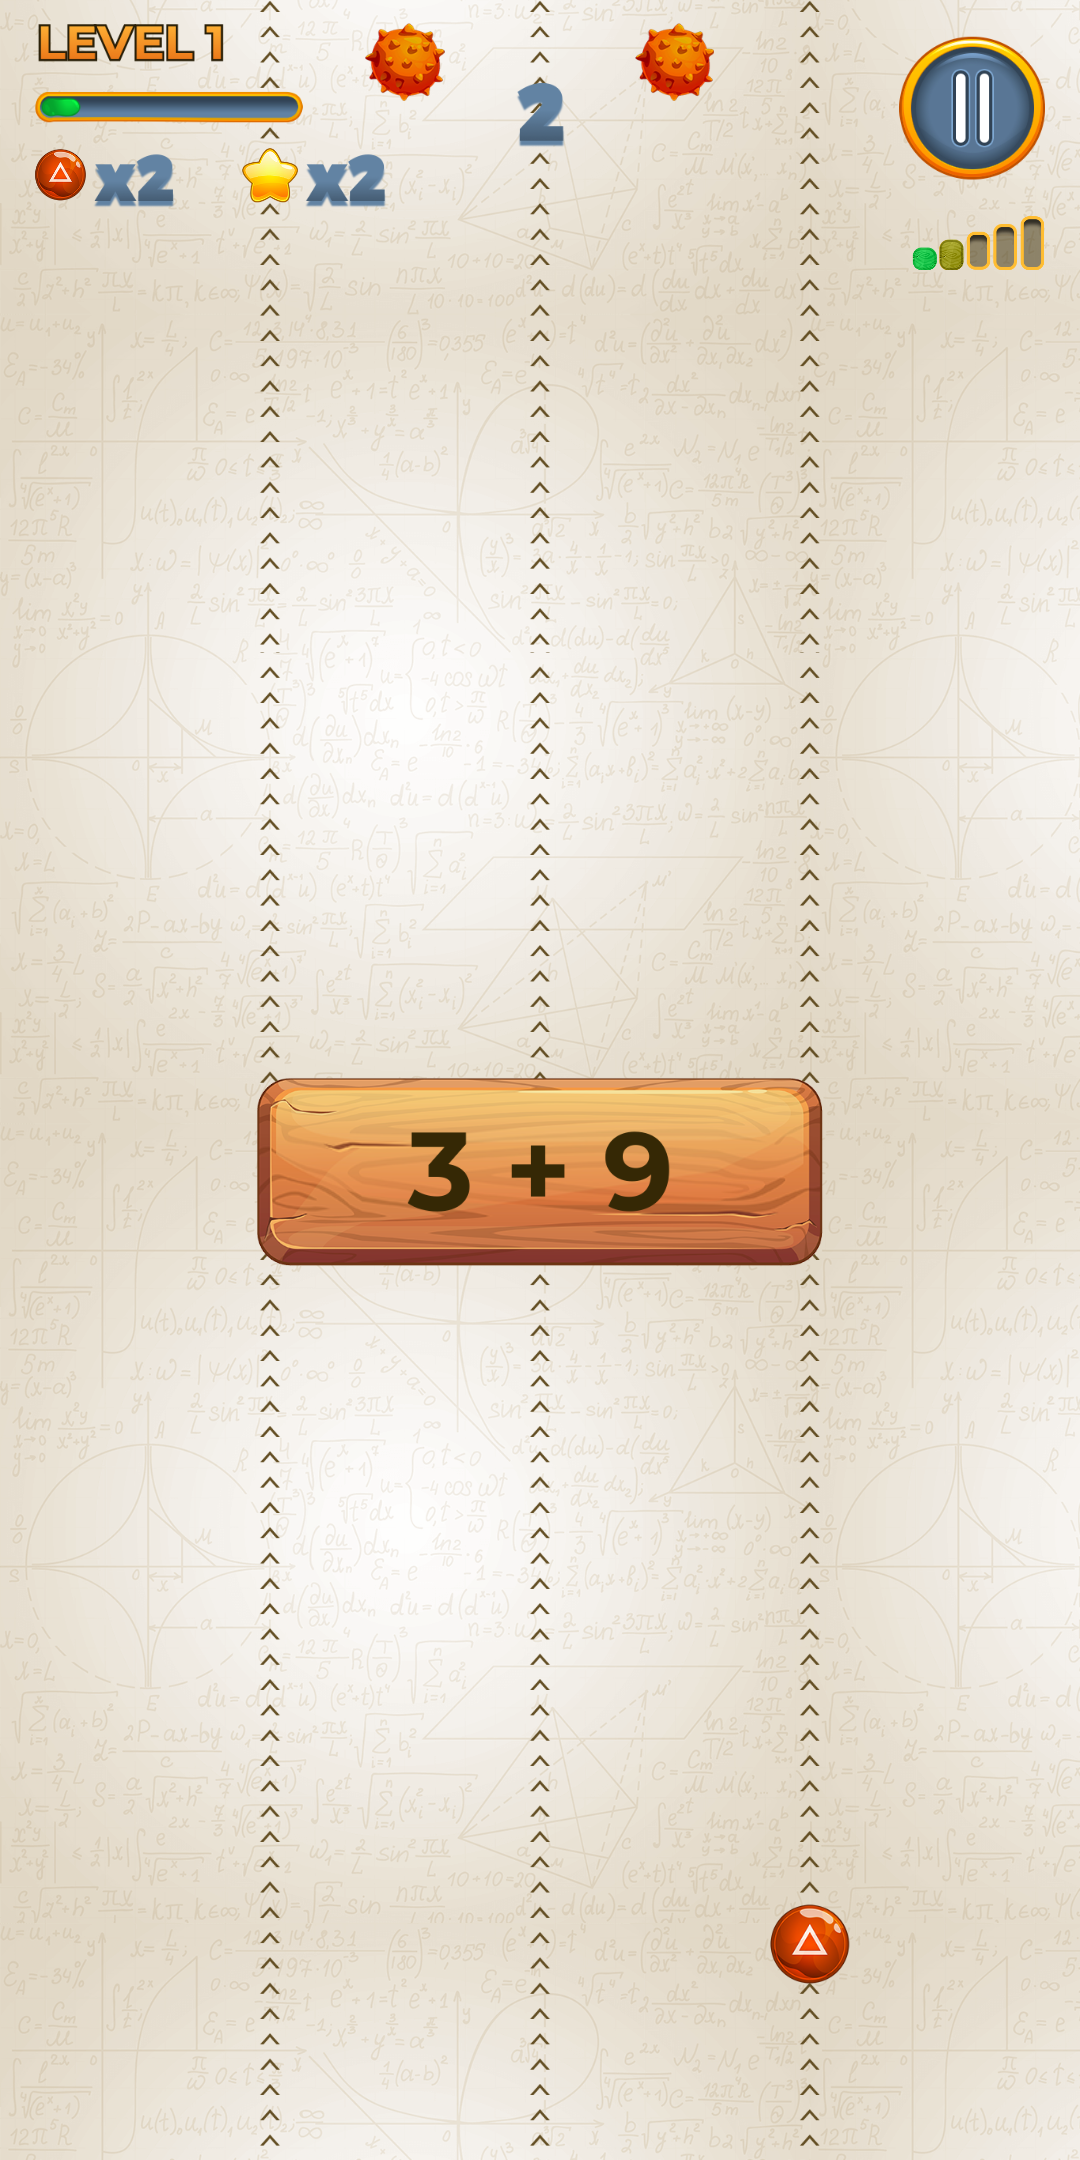
\includegraphics[scale=0.15]{"slike/igre/mathematicalrun1.png"} 
				\caption{Postavljen zadatak}
				\label{fig:zadatak}
			\end{minipage}\hfill
			\begin{minipage}{0.48\textwidth}
				\centering
				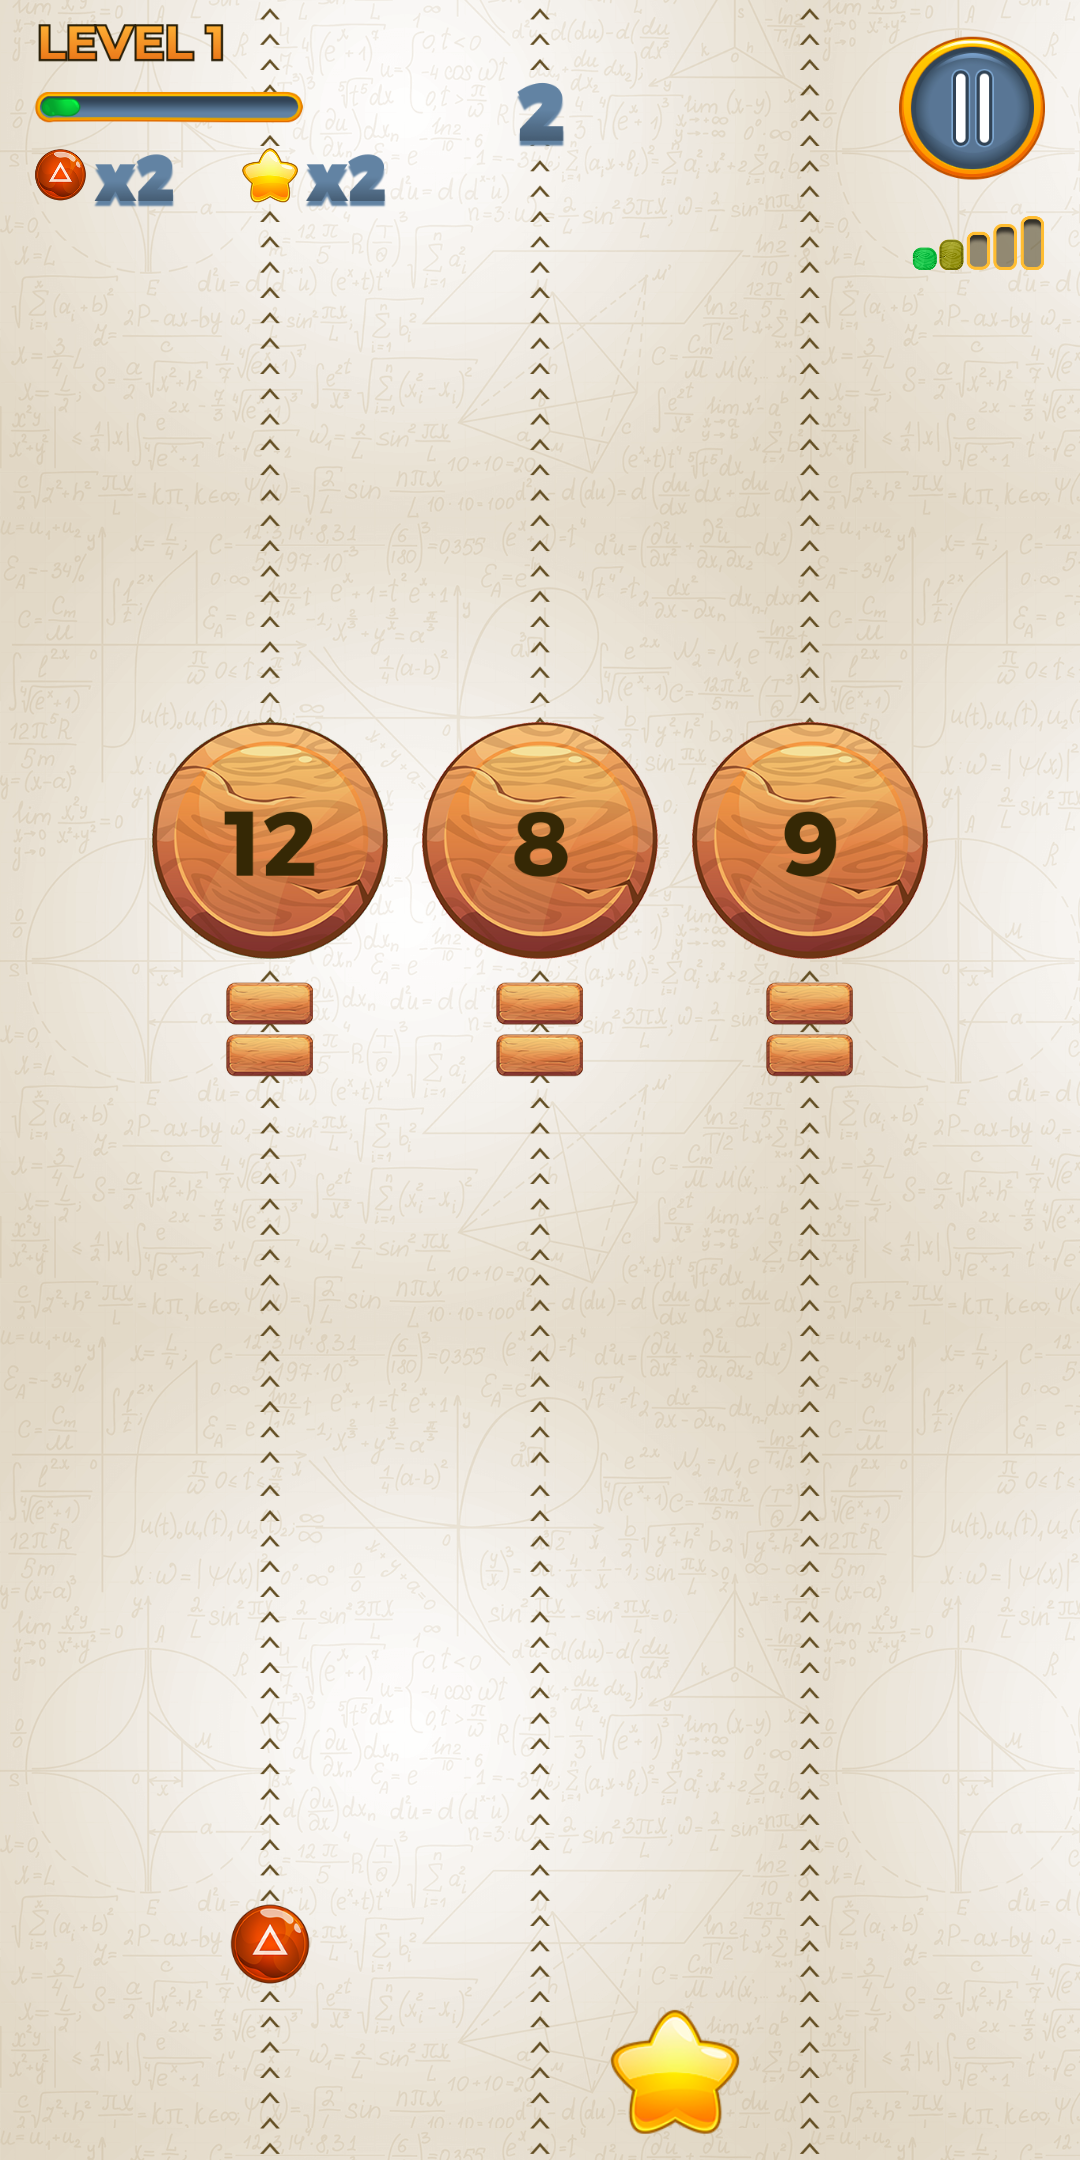
\includegraphics[scale=0.15]{"slike/igre/mathematicalrun2.png"} 
				\caption{Ponuđeni odgovori}
				\label{fig:odgovori}
			\end{minipage}
		\end{figure}

Igrica omogućava odabir tipa zadataka, odnosno zadatak tipa "skupljaj parne brojeve", zadatak tipa "skupljaj manje od x" no ne i sve te zadatke na način da se izmijenuju, već igrač može igrati isključivo jedan zadatak "at the time", tada se na ekranu 
prikazuju samo odgovori, no način igranja je i dalje isti; 3 trake sa neresponzivnim kontrolama. Ova igrica je potencijalno "endless runner". 

\chapter{Korištene tehnologije}
U sklopu ovog rada korištena je nekolicina različitih tehnologija. Dok su odabrane opisane u nastavku, valja naglasiti da ove tehnologije nisu nužno najbolje. U svrhu izrade ovog rada birane su tehnologije koje su prikladnije za samu kompleksnost izrade rada.
Konkretnije, korištenje poznatog pokretačkog stroja (engl. \textit{game engine}) Unity značajno bi olakašlo izradu igre. Jedan od takvih primjera opisan je u poglavlju 5.1. "Implementacija mobilne igre - Pozadina". 
U sklopu ovog rada programski jezik Java jedini je jezik koji se koristi za potrebe izrade mobilne igre. Iako je mobilna igra djelomično samostalna, odnosno ne treba joj web poslužitelj kako bi se mogla igrati sa pretpostavljenim postavkama, za potrebe 
preuzimanja postavki i slanja rezultata igre učiteljici koristi se Node.js server. Ovaj server koristi se i za potrebe web stranice, dok je sam prikaz web stranice napravljen korištenjem EJS.


	\section{Java}
	Java je objektno orijentirani programski jezik objavljen krajem 1995. kada tvrka Sun Microsystems objavljuje prvu verziju ovog programskog jezika. Programski jezik java ozmišljen je, odnosno njegova je ideja i velika prednost platformska neovisnost,
	što znači da se jednom prevedeni programski kod može pokrenuti na bilo kojem sustavu, odnosno računalu. No, ovo za sobom povlači to da se program ne može direktno prevesti u strojni kod određenog procesora, već na svakom računalu treba biti
	instalirana podrška za izvođenje Java programa (JVM - Java Virtual Machine). 
	Jedna od prednosti programskog jezika Java je i ta da uz to što jezik biva kontinuirano nadograđivan, generalno je unatrag kompatiblan (engl. \textit{backwards compatible}), što znači da će se jednom napisani kod moći pokrenuti i nakon nove nadogradnje.
	Kao česti nedostatak programskog jezika Java navodi se "verbosity" odnosno opširnost pisanja koda, koju ja osobno smatram kao prednost jer u konačnici pruža preglednost koda i lakše razumijevanje, čemu doprinosi i statičko tipiziranje, odnosno 
	potreba za navođenjem svakog tipa podatka eksplicitno. 
	
	Programski jezik Java veliku popularnost doživljava pojavom Android uređaja, gdje je dugotrajni niz godina bio glavni jezik za razvoj aplikacija. Prethodnih godina, veliki zamah za razvoj android mobilnih aplikacija doživljava programski jezik 
	Kotlin koji se u konačnici oslanja na JVM, no uvodi razne sintaksne pokrate. 
	
	
	
	\section{Node.js}
	Node.js je \textit{open-source, cross-platform, back-end JavaScript runtime} okruženje i izvršava JavaScript kod izvan web-preglednika. "Node.js je incijalno napisan od strane  Ryan Dahl u 2009. godini, otprilike 13 godina poslije predstavljanja
	prvog  \textit{server-side} Javascript okruženja." [SAD OVDJE LINK NA IZVOR] (wiki, node.js)
	
	Node.js omogućava jednostavnu izradu Web servera i drugih mrežnih alata korištenjem JavaScripta uz razne biblioteke. Iako Node.js nativno podržava samo JavaScript, programski kod je moguće pisati i u programskim jezicima koju su prevodivi u JavaScrpt kao 
	što je to npr. TypeScript, odnosno Dart. Node.js koristi skriptiranje na poslužiteljskoj strani; što znači da se skripte pokreću na poslužitelju, gdje se i generira dinamički sadržaj web stranice koji se potom šalje korisnikovom web pregledniku. 
	Konkretnije, u sklopu ovog projekta korišten je Express.js koji je okvir/kostur (engl.\textit{framework}) izgrađen na bazi Node.js. Ovaj kostur dodatno pojednostavljuje odnosno nudi razne akcije kao što su različite metode HTTP zahtjeva (GET, POST,...).
	
	
	\section{HTML, CSS, EJS}
	HTML je jezik za označavanje (engl. \textit{markup}) koji opisuje strukturu web stranice koju web preglednici koriste za strukturirani prikaz web stranice. HTML elementi su elementi za koje se može reći da predstavljaju blokove koje je moguće slagati
	i ugnježđavati jedan unutar drugoga. HTML pruža semantiku kako za oblikovanje teksta tako i za direktan unos sadržaja na stranicu poput slika.
	Dva su glavna tipa oznake; prvi tip je takav da okružuje tekst. Npr sa: 
		\begin{lstlisting}[language = HTML , frame = trBL , firstnumber = 1 , escapeinside={(*@}{@*)}]
		<h1> Naslov </h1>
		\end{lstlisting}
		definirao bi se prikaz jednog naslova. Element se otvara oznakom "<h1>" poslije koje slijedi sadržaj koji se u konačnici zatvara sa "</h1>. Drugi tip elementa je samozatvarajuć kao što je "<br />" koji predstavlja prelom retka.

	HTML kao jezik veoma je ograničen jezik kada se govori o stiliziranju te se za te potrebe koristi jezik CSS. CSS je jezik koji dodatno opisuje kako se određeni elementi trebaju prikazivati. Neke od primjena CSSa je opisivanje boja, pozadina, obruba,
	margina, raznih udaljenosti, širine, visine, poravnanja, fontova i raznih drugih detalja. CSS kod može se izravno postavljati na svaki element, može se definirati unutar iste datoteke ili se može uključiti kao vanjska biblioteka. 
	
	\textit{Embedded JavaScript templates} (nadalje EJS) je jednostavan i elegantan jezik za pisanje HTML predložaka koristeći čisti JavaScript kod. Prilikom izvođenja EJS izvodi dio JavaScript koda kao što i zamijenuje varijable stvarnim vrijednostima te
	u konačnici stvara čistu HTML, CSS stranicu.
	

	

\chapter{Implementacija mobilne igre}

	\section{Pozadina}
	Pozadina je tematski zamišljena kao put iz središta zemlje  do dubokog svemira. Mobilna igra je takozvani endless runner, što znači da se potencijalno može igrati beskonačno,
	odnosno ne postoji način na koji igra završava osim u slučaja da igrač izgubi sve živote, stoga je osim samog efekta "putovanja ka svemiru" potrebno osigurati i beskonačno pomicanje same pozadine.
	
	Pozadina kao takva se u konačnici sastoji od 20ak slika čije spajanje vertikalno daje efekt kontinuiranosti. Dok poznati pokretački strojevi (engl. \textit{game engine}) poput Unity nudi opcije manipulacija
	pozadinom, kao što je beskonačno ponavljajuća pozadina, ta mogućnost u ovakvom razvoju aplikacije nije moguća, već ju je potrebno iskodirati samostalno. 
	Za početak je potrebno učitati slike pozadina kao Bitmap te ih omotati u objekte kako bi im se dala različita svojstva poput x i y koordinata gdje se trenutno nalaze. Takvi objekti pohranjeni su u polje.
	
	Radi jednostavnosti, svaka slika pozadine se  vertikalno i horizontalno skalira na broj piksela koje zaslon mobitela ima; zbog toga, u jednom trenutku na zaslonu se mogu vidjeti maksimalno dvije slike
	pozadine od jednom. Na samom početku igre uzimaju se prva dva objekta pozadine iz polja. Prvi objekt predstavlja donju pozadinu koja će biti prikazana, a drugi gornju pozadinu.  Donju pozadinu potrebno je inicijalizirati
	na lokaciju sa x koordinatom 0 i y koordinatom 0, odnosno želimo da se pokazuje od početka zaslona vertikalno i horizontalno. Drugu sliku inicijaliziramo opet tako da joj damo x koordinatu 0, no y koordinatu postavljamo
	na minus vertikalnu veličinu zaslona. Na svako ponovno osvježavanje igre, pozadina se vertikalno spušta ka dolje čime se stvara efekt putovanja igrača prema gore. Spuštanje pozadine prema dolje implementacijski je 
	ostvareno tako što se svakim osvježavanjem zaslona povećava y koordinata obje slike za određenu vrijednost, ovisno o tome kojom brzinom želimo da "igrač putuje ka svemiru". 
	
	Na sljedećoj slici može se vidjeti način iscrtavanja pozadine na ekranu i izvan njega.
	
	\begin{figure}[H]
			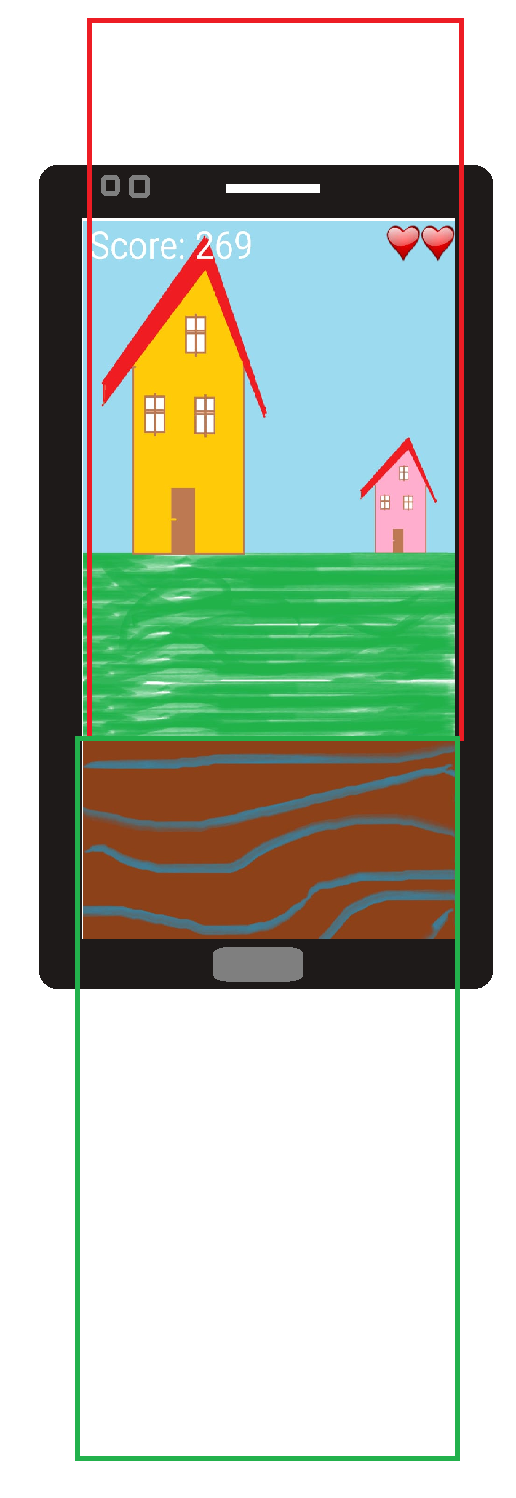
\includegraphics[scale=0.6]{"slike/background.png"} 
			\centering
			\caption{Pomicanje pozadine}
			\label{fig:pomicanjepozadine}
	\end{figure}
		

	
	U trenutku kada y koordinata donje slike izađe izvan ekrana (odnosno kada je vrijednost y osi veća od y dimenzije ekrana) nova donja slika sada je slika koja je bila gore, a novu gornju sliku uzimamo 
	kao sljedeći član polja. 
	Zadnja slika prikazuje svemir pun zvijezdi i nju u polje učitavamo dva puta (dva različita objekta). U trenutku kad smo u igri došli do te slike, tim dvijema slikama se konstanto mijenjaju vrijednosti y osi.
	Odnosno kad donja slika izađe dolje s ekrana, ponovno se postavljaju vrijednosti y osi za obje slike. 
	
	
	Cijeli način implementacije pomicanja pozadine možemo prikazati sljedećim kodom:
	
	\begin{lstlisting}[language = Java , frame = trBL , firstnumber = 1 , escapeinside={(*@}{@*)}]
   private void updateBackground() {
        currentDownBackground.setY(currentDownBackground.getY() + 5);
        currentUpBackground.setY(currentUpBackground.getY() + 5);

        if (currentDownBackground.getY() > screenY) {
            currentDownBackground = currentUpBackground;
            if (currentBackgroundIndex < backgrounds.length - 1)     
                currentUpBackground = backgrounds[++currentBackgroundIndex]; 
            else {
                currentDownBackground = backgrounds[backgrounds.length - 2];
                currentDownBackground.setY(0);
                currentUpBackground = backgrounds[backgrounds.length - 1];
            }
            currentUpBackground.setY(-screenY);
        }
    }
	\end{lstlisting}


	\section{Objekt za skupljanje}
	Slično kao i pozadinu, objekt koji se kontrolira, odnosno objek s kojim se skupljaju padajući objekt učitan je kao kao Bitmap, odnosno više njih, konkretnije kao dva Bitmap objekta omotana sa objektom
	klase "Saw". Za razliku od pozadine koja je putovala prema dolje, objekt s kojim skupljamo padajuće objekte je statičan na ekranu, odnosno ne mijenja svoj položaj na ekranu bez korisničke akcije. Pod kornisničku akciju u 
	ovom slučaju podrazumijeva se dodir ekrana. Koristeći oblikovni obrazac promatrač (engl. \textit{observer}), pri inicijalizaciji igre  subjektu (objektu konkretne klase "View", u ovom slučaju to je "SurfaceView")
	se postavlja konkretna implementacija apstraktnog promatrača "OnTouchListener". Navedeno sučelje sastoji se od jedne funkcije:
	\begin{lstlisting}[language = Java , frame = none , numbers=none, escapeinside={(*@}{@*)}]
		boolean onTouch(View v, MotionEvent event); 
	\end{lstlisting}
	
	Ova funkcija prima dva parametra, "View v" koji je pokazivač na "View" kojem je događaj dodira dostavljen te parametar "MotionEvent event" koji opisuje tip događaja. Primjeri tipova događaja su: 
	"ACTION\_DOWN" koji govori da se dogodio pritisak na zaslonu, "ACTION\_UP" koji govori da je dodir zaslona otpušten, "ACTION\_MOVE" koji govori da se dogodila promjena pozicije između pritiska ("ACTION\_DOWN") i otpuštanja
	("ACTION\_UP") te nekolicina raznih drugih akcija. Navedena funkcija vraća primitivni tip boolean koji u ovom slučaju predstavlja zastavicu koja govori da li je konkretni promatrač "konzumirao događaj do kraja".
	
	U nastavku je prikazan cijeli programski kod potreban za pomicanje objekta za skupljanje. Konkretna implementacija sučelja "OnTouchListener" izvedena je kao anonimni razred, odnosno zbog bolje preglednosti koda 
	koristi se pokrata u vidu lambda izraza, dok "this" predstavlja objekt klase View.

		\begin{lstlisting}[language = Java , frame = trBL , firstnumber = 1 , escapeinside={(*@}{@*)}]
			 this.setOnTouchListener((v, event) -> {
            if (event.getAction() == MotionEvent.ACTION_MOVE 
					|| event.getAction() == MotionEvent.ACTION_DOWN) {
                saw.setX((int) event.getX());
            }
            return true;
        });
		\end{lstlisting}
		
	Na ovom programskom kodu potrebno je uočiti da se kontroliranje našeg objekta može dogoditi doticanjem i pomicanjem prsta na bilo kojem dijelu ekrana, no da sam objekt kojeg kontroliramo neće promijeniti 
	vrijednost svoje x osi, odnosno neće se pomicati vertikalno, već se isključivo mijenja vrijednost položaja na horizontalnoj osi; također je bitno uočiti da za pomicanje objekta nije potrebno stisnuti na objekt
	te ga povući, već je dovoljno stisnuti na određeno mjesto na ekranu te će se objektov položaj na horizonalnoj osi teleportirati na željeno mjesto. Iako je ovo programsko riješenje vjerojatno najjednostavnije, 
	kasnije će se ispostaviti da je ujedno i najbolje. Ukratko, može se dogoditi da objekt kojeg kontroliramo bude okružen s padajućim objektima koji se ne smiju pokupiti i stoga je ova mogućnost "teleportiranja" poželjna.
	
	
	Kao što je već ranije navedeno, objekt za skupljanje koji se kontrolira ne mijenja svoj položaj na ekranu (bez prethodne akcije korisnika) već je potreba učitavanja više slika, odnosno stvaranja više Bitmap 
	objekata nastala u svrhu stvaranja animacije. Animacija se stvara tako što se brzo izmijenjuju slike koje se iscrtavaju na zaslonu. Konkretno, ova animacija sastoji se od dvije slike koje se neprestano izmijenuju.
	Prva slika nastala je jednostavnim crtanjem, dok je druga nastala rotacijom za određeni kut te dodavanjem dodatnih detalja. 
	
	Sljedeće dvije slike prikazuju objekt s kojim skupljamo padajuće objekte, odnosno zajedno prikazuju oštricu koja se rotira velikom brzinom.
	
	
		\begin{figure}[!htb]
			\begin{minipage}{0.48\textwidth}
				\centering
				
\includegraphics[scale=0.6]{"slike/saw1.png"} 
				\caption{Originalna slika oštrice}
				\label{fig:saw1}
			\end{minipage}\hfill
			\begin{minipage}{0.48\textwidth}
				\centering
				
\includegraphics[scale=0.6]{"slike/saw2.png"} 
				\caption{Zarotirana originalna slika oštrice sa dodatnim detaljima}
				\label{fig:saw2}
			\end{minipage}
		\end{figure}
	
	\section{Padajući objekti}
	Padajući objekti implementirani su kao apstraktna klasa "FallingObject" čije su konkretne implementacije "Square" (kvadrat) i "Circle" (Krug). Ova apstraktna klasa definira nekolicinu zajedničkih vrijednosti, 
	odnosno vrijednost koju treba imati svaki padajući element kao što su položaj padajućeg objekta, njegova boja, brzina i slično.
	Brzina je slučajna vrijednost koja je padajućem objektu pridjeljena prilikom stvaranja te ona iznosi između X i X + slučajan broj između 0 i 10, gdje X označava minimalnu brzinu kojom objekt pada i ta vrijednost
	varijable X ovisi o trenutnoj težini igre, odnosno iznosi 5 na samom početku igre. Taj broj, slično kao i spuštanju pozadine označava za koliku udaljenost će se ovaj objekt pomaknuti prema dolje svakim osvježavanjem ekrana.
	Uz to nudi i razne konkretne implementacije metoda te metode koje različite konkretne implementacije ove apstraktne klase trebaju nadjačati, odnosno ponuditi svoje implementacije. 
	
	
		\begin{figure}[!htb]
			\begin{minipage}{0.48\textwidth}
				\centering
				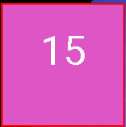
\includegraphics[scale=0.6]{"slike/square.png"} 
				\caption{Primjer padajućeg objekta - Kvadrat}
				\label{fig:squre}
			\end{minipage}\hfill
			\begin{minipage}{0.48\textwidth}
				\centering
				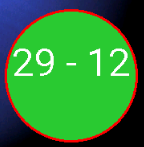
\includegraphics[scale=0.6]{"slike/circle.png"} 
				\caption{Primjer padajućeg objekta - Krug}
				\label{fig:circle}
			\end{minipage}
		\end{figure}
		
		Generalno govoreći jedina razlika između ove dvije konkretne implementacije abstraktne klase "FallingObject" je sami oblik padajućeg objekta i način na koji ih opisujemo, stoga se abstraktne metode metode također odnose na sami oblik objekta.
		Tu su najznačanije dvije metode, jedna služi za samo iscrtavanje objekta na ekranu, dok druga provjerava da li se taj objekt i objekt za skupljanje drugih objekta preklapaju. Odnosno provjerava da li je korisnik skupio padajući objekt.
		Sadržaj svakog padajućeg objekta ovisi o trenutnom zadataku. 
		
	\subsection{Provjera kolizije - Kružnica}
	S obzirom da je padajući objekt "Circle" pa tako i sam objekt s kojim skupljamo padajuće objekte kružnog oblika, koliziju ovih objekta provjerava se čistim matematičkim putem. 
	
		\begin{figure}[H]
			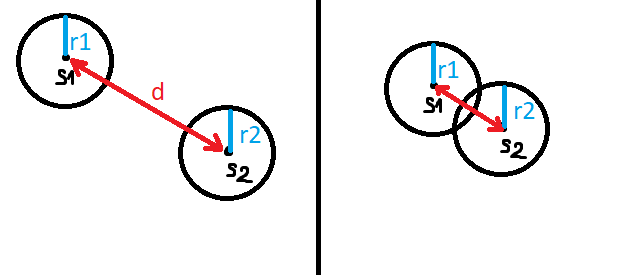
\includegraphics[scale=0.6]{"slike/circlekolizija.png"} 
			\centering
			\caption{Provjera kolizije za objekte kružnog oblika}
			\label{fig:kolizijacircle}
		\end{figure}
	
	Na lijevom dijelu slike vidimo dva objekta koja se ne preklapaju. To matematičkim putem dokazujemo na način da pokažemo da kvadrat udaljenosti središa ova dva objekta nije manji ili jednak kvadratu sume radiusa. Analogno, na desnom dijelu slike
	mogu se vidjeti dvije kružnice koje imaju točke preklapanja i za njih se može vidjeti da je kvadrat udaljenost središta manji no kvadrat sume radiusa. 
	
	\subsection{Provjera kolizije - Kvadrat}
	Provjera objekta s kojim skupljamo padajuće objekte i kvadrata kao padajućeg objekta više se ne može provjeriti na isti način kao i za kružnicu jer se ovaj problem svodi na preklapanje kružnice i kvadrata.
	Ovaj problem generalno se ne može na lijep način prikazati matematički već je u ovom slučaju implementiran tako da se uzme 8 točaka s objekta s kojim skupljamo padajuće objekte i za svaku od tih 8 točaka provjeravamo nalazi li se unutar 
	kvadrata (padajućeg objekta). Ukoliko se samo jedna točka nalazi unutar kvadrata dva objekta se preklapaju. 
	
			\begin{figure}[H]
			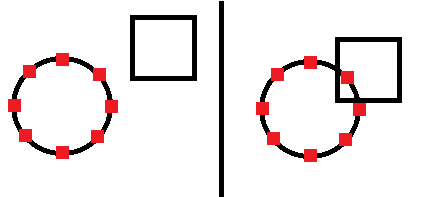
\includegraphics[scale=0.6]{"slike/squarekolizija.png"} 
			\centering
			\caption{Provjera kolizije za objekte oblika kvadrata}
			\label{fig:kolizijasquare}
		\end{figure}
		Na lijevom dijelu slike prikazani su objekti koji se ne preklapaju. Dok se na desnom dijelu slike vide dva objekta koja se preklapaju što je u igri dokazano tako što je pokazano da je jedna od točaka objekta za skupljanje unutar padajućeg kvadrata.
	
	\section{Zadaci}
	Zadaci su definirani apstraktnom klasom "Task". Ova klasa u sebi čuva tekst zadatka te najvažnije nudi metode koje svaki konkretni zadatak treba nadjačati. Gdje su najznačanije sljedeće metode:
	\begin{lstlisting}[language = Java , frame = trBL , firstnumber = 1 , escapeinside={(*@}{@*)}]
	public abstract boolean checkCollectedIsValid(FallingObject fallingObject);
	public abstract FallingObject makeFallingObject();
	\end{lstlisting}
	Konkretne implementacije ove apstraktne klase trebaju ponuditi svoje implementacije
	 ovih metoda tako da metoda "checkCollectedIsValid" za primljeni padajući objekt (fallingObject) provjerava da li je skupljeni objekt u skladu sa postavljenim zadatkom ovisno o tome kako je definiran sam konkretni
	 zadatak. Slično tome, metoda "makeFallingObject" stvara padajući objekt na zahtjev;  sadržaj tog padajućeg objekta ovisiti će o trenutnom zadatku. Izvedena su 4 osnovna (primitiva) tipa zadatka iz komponente "Task"
	 "NumberTask" koji se nadalje dijeli na "RelativeNumberTask" i "UnrelativeNumberTask", "ShapeTask" te "WordsTask". Osim osnovnih tipova zadatak definiran je i "ComplexTask"  koji je zapravo predstavlja kompozit (grupu)
	 osnovnih tipova zadatak.
	 Tip zadatka "RelativeNumberTask" definiran je sa donjom i gornjom granicom iz koje će se brojevi generirati, relativnim brojem, tj. brojem u odnosu na kojeg će se operacija gledati, samom operacijom te
	 zastavicom koja govori mijenja li se relativan broj nakon promjene zadatka. Ukoliko je zastavica postavljena nakon promjene zadatka novi relativni broj bit će slučajni broj iz zadanog raspona. Tip zadatka
	 "UnelativeNumberTask" generalno je sličan tipu zadatka "RelativeNumberTask" no ovaj tip zadatka jednostavno nema relativan broj. Primjer tipa "ShapeTask" zadatka je "Skupljaj kvadrate", odnosno jednostavno ovisi
	 o obliku padajućeg objekta. Tip zadatka "WordsTask" omogućava zadatke poput "Skupljaj geometrijske likove" tako što u konstruktoru prima dvije liste riječi. Listu riječi koja sadržava ispravne odgovore i listu riječi
	 koja sadrži neispravne odgovore. 
	 
	 Kompozit "ComplexTask" se koristi za kombiniranje zadataka i primjer takvog zadatka bio bi "Skupljaj brojeve veće od X koji su u kvadratu", tj. ovaj zadatak se sastoji od dva osnovna tipa zadatka, tj.
	 "RelativeNumberTask" (brojevi veći od X) i "ShapeTask" (u kvadratu). Kako bi skupljeni padajući objekt bio korektno skupljen svaki od zadataka treba biti ispunjen. To se postiže delegacijom operacija na primitivne
	 komponente, odnosno sastavne komponente (djecu) tog kompozita.
	
	\begin{lstlisting}[language = Java , frame = trBL , firstnumber = 1 , escapeinside={(*@}{@*)}]
	 @Override
    public boolean checkCollectedIsValid(FallingObject fallingObject) {
        for (Task task : tasks) {
            if (!task.checkCollectedIsValid(fallingObject)) return false;
        }
        return true;
    }

    @Override
    public FallingObject makeFallingObject() {
        int randomTask = (int) (Math.random() * tasks.size());
        return tasks.get(randomTask).makeFallingObject();
    }
	\end{lstlisting}
	
	\section{Prilagođavanje težine}
	Za prilagodbu težine igre koristi se veoma jednostavan algoritam. Padajući objekti imaju određenu brzinu padanja kao što je navedeno u poglavlju koji ih opisuju. Osim toga, zadana je i početna vjerojatnost 
	s kojom će se pojaviti padajući objekt koji nema prikazan broj direktno, već matematički izraz. Osim toga, promijenjiva je i frekvencija kojom se padajući objekti stvaraju. Svaki dobro sakupljenim padajućim objektom
	slučajnim odabirom bira se način otežavanja igre. Odnosno, ukoliko igrač pokupi ispravan padajući objekt igra će slučajnim odabirom odabrati hoće li ubrati stvaranje padajućih objekata ili će povećati minimalnu brzinu
	s kojom padajući objekti padaju ili će povećati vjerojatnost pojavljivanja izraza.
	Suprotno tome ukoliko igrač ne uspije pokupiti padajući objekt osim što će izgubiti određeni broj bodova, igra će se olakšati slučajnim odabirom. Za kraj, ukoliko igrač pokupi padajući objekt koji nije trebao, osim što će
	izgubiti život igra će se značajnije olakšati, odnosno smanjiti će se minimalna brzina padajućeg objekta kao i frekvencija stvaranja objekata pa tako i vjerojatnost pojavljivanja izaza.
	
	
	\section{Komunikacija sa poslužiteljom}
	Komunikacija sa poslužiteljem ostvarena je koristeći Java klasu "HttpURLConnection". Od generalnih implementacijskih detalja potrebno je glasiti da se sav mrežni promet mora odvijati na sporednoj dretvi. 
	Podaci koji se šalju s mobitela na poslužitelj šalju se u obliku JSON (JavaScript Object Notation). U sklopu ovog projekta nisu korištenje vanjski \textit{dependency} poput "GSON", već
	su napisane funkcije potrebne za izradu i tumačenje svakog JSON zapisa koji se može koristiti. U sljedeća dva potpoglavlja opisani su neki detalji o tome.
	\subsection{Dohvat zadataka}
	Dohvat zadataka odnosi se na preuzimanje postavki koje su generirane putem web stranice. GET zahtjevom na poslužitelj programskim kodom dohvaća se JSON kojeg mobilna aplikacija prepozaje kao običan tip "String".
	Navedeni GET zahtjev radi se na bazni URL koji je u ovom slučaju "https://denismath .herokuapp.com/gamecode/mobile/" na koji se dodaje ono što funkcija "getMethod" primi. Npr. Ukoliko korisnik mobilne igre želi preuzeti postavke
	igre koje imaju kod "123456"  taj parametar bit će "settings/123456"; odnosno GET zahtjev otići će na "https://denismath.herokuapp.com/gamecode/mobile/ settings/123456".
	Jednom dohvaćene postavke spremaju se u memoriju mobilnog uređaja u obliku tipa String. Pri pokretanju zaslona u kojem igra dohvaćaju se postavke iz memorije te se njihovim tumačenjem stvaraju Java objekti koji predstavljaju zadatke.
	Ovi objekt spremaju se u listu iz koje će kasnije igra slučajnim odabirom odabirati trenutni zadatatk. Tumačenje preuzetih postavki i generiranje Java objekata svodi se na "lomljenje" sadržaja spremljene String varijable
	na zadatke koji su bili odvojeni određenim znakovnim nizom, što je u ovom slučaju "\#DELIMITER\#".
	Za postavke zapisane u obliku:
	
	
	\begin{lstlisting}[language = Java , frame = trBL , firstnumber = 1 , escapeinside={(*@}{@*)}]
	taskObjectType:RelativeNumberTask;taskText:Manjiod;taskType:lower;minNumber:-5;maxNumber:55;relativeNumber:21;allowRelativeNumberChange:0#DELIMITER#taskObjectType:WordsTask;taskText:geometrijske likove;taskType:WORDCONTAINED;correctWords:kruznica,trokut,kvadrat;incorrectWords:piramida,valjak,sfera
	\end{lstlisting}
	s ovim postupkom dobivamo sljedeće zapise koje je nadalje potrebno tumačiti.
	\begin{lstlisting}[language = Java , frame = trBL , firstnumber = 1 , escapeinside={(*@}{@*)}]
	taskObjectType:RelativeNumberTask;taskText:Manjiod;taskType:lower;minNumber:-5;maxNumber:55;relativeNumber:21;allowRelativeNumberChange:0
	taskObjectType:WordsTask;taskText:geometrijske likove;taskType:WORDCONTAINED;correctWords:kruznica,trokut,kvadrat;incorrectWords:piramida,valjak,sfera
	\end{lstlisting}
	Ovaj postupak tumačenja nadalje je jednostavan. Potrebno je tekst rastaviti po točka-zarez, čiji bi rezultat temeljem prvog zapisa bio
	\begin{lstlisting}[language = Java , frame = trBL , firstnumber = 1 , escapeinside={(*@}{@*)}]
	taskObjectType:RelativeNumberTask
	taskText:Manjiod;taskType:lower
	minNumber:-5;maxNumber:55
	relativeNumber:21
	allowRelativeNumberChange:0
	\end{lstlisting}
	Ovaj sadržaj sada se rastavlja po znaku dvotočke te se sav sadržaj dodaje u Map<String,String> gdje je ključ sadržaj prije dvotočke, dok je vrijednost jednaka sadržaju poslije dvotočke.
	Iz ove mape nadalje je trivijalno izraditi objekt tipa "RelativeNumberTask" koji predstavlja zadatak. 


	\subsection{Slanje rezultata igre}
	Slanje rezultata sličan je proces dohvatu zadataka, no ovog puta se sadržaj šalje u obliku JSON objekta kojeg je potrebno generirati te se ovo slanje rezultata izvod pomoću metode POST. 
	Za potrebe izvođenja POST metode koristi se funkcija "postMethod" koja prima dodatak koji se pridodaje na bazni link tipa String te Map<String, String> koji sadrži sve podatke. 
	Izrada cijelog JSON objekta napravljena je sljedećim programskim kodom:
	\begin{lstlisting}[language = Java , frame = trBL , firstnumber = 1 , escapeinside={(*@}{@*)}]
	  StringBuilder makingJson = new StringBuilder();
            makingJson.append("{");

            for (Map.Entry<String, String> keyvalue : body.entrySet()) {
                if (!keyvalue.getValue().startsWith("[")) {
                    makingJson.append("\"")
					.append(keyvalue.getKey())
					.append("\":\"")
					.append(keyvalue.getValue())
					.append("\",");
                } else {
                    makingJson.append("\"")
					.append(keyvalue.getKey())
					.append("\":")
					.append(keyvalue.getValue())
					.append(",");
                }

            }
            //makni zadnji zarez
            makingJson = new StringBuilder(
				makingJson.substring(0,makingJson.length() - 1));
            makingJson.append("}");
	\end{lstlisting}
	
	
	
\chapter{Implementacija poslužitelja i web stranice}
	\section{Izrada web servera}
	Kao što je već ranije navedeno u sklopu ovog projekta za izradu web poslužitelja korišten je Express.js koji je kostur na bazi Node.js. Ova tehnologija omogućava izradu web poslužitelja u svega par linija koda.
	\begin{lstlisting}[language = Java, frame = trBL , firstnumber = 1 , escapeinside={(*@}{@*)}]
	const express = require('express');
	const app = express();
 
	// Postavljanje EJS
	app.set('view engine', 'ejs');
 
	app.get('/', function (req, res) {
    res.send('Hello World');
	})

	app.listen(3000);
	\end{lstlisting}
	
	Pokretanjem ovog programskog koda moće će se pristupiti web serveru koji će se nalaziti na adresi localhost:3000. Sve što je dalje potrebno je napisti funkcionalnosti pristupnih točaka (engl. \textit{endpoint}).

	\section{Izrada pristupnih točaka}
	Radi modularnosti programskog koda  pristupne točke grupirati će se u različite module koji koriste express.Router(). Jedan od napisanih modula tako je modul koji se koristi pri logiranju i on se sastoji od dvije pristupne točke. Jedna koristi HTTP metodu get, dok druga koristi metodu POST.
	\begin{lstlisting}[language = Java, frame = trBL , firstnumber = 1 , escapeinside={(*@}{@*)}]
	router.get('/', function (req, res, next) {
		if (req.session.user !== undefined) {
			return res.redirect('/');
		}

		res.render('login', {
			title: 'Login',
			linkActive: 'login',
			err: undefined,
		});
	});
	\end{lstlisting}
	
	Prikazani kod pruža sljedeću funkcionalnosti: provjerava da li je korisnik već ulogiran te ako je preusmjerava ga na početnu stranicu. Ukoliko korisnik nije ulogiran koristeći EJS i definirani pogled (engl. \textit{view}) korisniku se vraća
	web stranica sa formom za login. Provjeru da li je korisnik ulogiran radi se pomoću sjednica (engl. \textit{session}) koje je također potrebno uključiti u projekt. Nakon što korisnik popuni i potvrdi formu s metodom post radi se HTTP zahtjev 
	na drugu pristupnu točku koja pak provjerava da li korisnik postoji, je li korisnik unesao ispravnu lozinku i slično te ovisno o ispravnosti korisničkog imena/lozike vraća odgovarajuću web stranicu pogreške, odnosno preusmjerava na početnu stranicu
	ukoliko je ulogiravanje bilo uspiješno. Ovdje je potrebno naglasiti da za provjeru ispravnosti korisničkog imena i lozinke poslužitelj poslužitelj podatke dohvaća iz baze podataka s kojom je također potrebno definirati vezu i napsati odgovarajuće SQL
	upite. 
	

	\section{Upotreba EJS}
	Ovaj pogled (engl. \textit{view}) za prijavu nije previše zanimljiv jer je njegov kod većinom čisti HTML te nema previše dinamičke izrade stranice. Jednostavnost, tj. lakoću korištenja EJS može se vidjeti na sljedećem programskom isječku koji 
	generira prikaz rezultata jedne igre, odnosno zapise o igri u obliku retka HTML tablice. 
	\begin{lstlisting}[language = HTML, frame = trBL , firstnumber = 1 , escapeinside={(*@}{@*)}]
	<% 	for(let rezultat of results){ %>
			<tr>
				<td><%= rezultat.player_nickname %></td>
				<td><%= rezultat.time %></td>
				<td><%= rezultat.highscore %></td>
				<td><a class="btn link" href="/gamecode/display/details/<%= rezultat.result_id %>"> See details</a></td>
            </tr>
	<% } %>
	\end{lstlisting}
	
	\section{Pristupne točke za spjanje na poslužitelj preko mobilne aplikacije}
	Pristupne točke za dohvaćanje podataka na mobilni uređaj slično su definirane kao i pristupne točke koje se koriste za web stranicu, no one umjesto da koriste EJS i vraćaju prikaz web stranice jednostavno vraćaju podatke u određenom obliku koji se potom tumače na
	mobitelu.
	Sljedeći progrogramski isječak definira pristupnu točku za dohvat postavki za određen id
	\begin{lstlisting}[language = Java, frame = trBL , firstnumber = 1 , escapeinside={(*@}{@*)}]
	router.get('/mobile/settings/:id', async function (req, res, next) {
		let gameCodeSettings;

		await (async () => {
			gameCodeSettings = await Setting.getGameCodeSettingsMobile(req.params.id);
		})();

		return res.send(gameCodeSettings);
	});
	\end{lstlisting}
	
	Statička metoda getGameCodeSettingsMobile dohvaća podatke iz baze podataka, formatira ih u željeni oblik koji opisan u podpodpoglavlju "Dohvat zadataka" te ih vraća mobilnom uređaju.
	\begin{lstlisting}[language = Java, frame = trBL , firstnumber = 1 , escapeinside={(*@}{@*)}]
    static async getGameCodeSettingsMobile(game_code) {
        try {
            let rezultat = await dbGetGameCodeSettingsMobile(game_code);
            rezultat = rezultat.rows;

            let formatiraniRezultat = "";
            for (let i = 0; i < rezultat.length; ++i) {
                formatiraniRezultat += rezultat[i].setting_text;
                formatiraniRezultat += "#DELIMITER#";
            }
            formatiraniRezultat.replaceAll("\n", "")
            return formatiraniRezultat;
        } catch (err) {
            console.log("ERROR getting game settings : " + JSON.stringify(this));
            throw err;
        }
    }
	\end{lstlisting}
	Dohvaćanje podataka iz baze podataka napravljeno je metodom dbGetGameCodeSettingsMobile koja je definirana kao :
	\begin{lstlisting}[language = Java, frame = trBL , firstnumber = 1 , escapeinside={(*@}{@*)}]
	dbGetGameCodeSettingsMobile = async (game_code) => {
		const sql = `SELECT *
					FROM setting
					WHERE game_code = '${game_code}'
					and is_deleted = 0`;
		try {
			return await db.query(sql, []);
		} catch (err) {
			console.log(err);
			throw err
		}
	};
	\end{lstlisting}	
	
	

\chapter{Baza podataka}
	Baze podataka su organizirane kolekcija podataka koje omogućavaju laki pristup podacima, uređivanje podataka i upravljanje istih. U sklopu ovog projekta koristio se
	SQL tip baze podataka, konkretnije PostgreSQL. PostgreSQL je besplatni, open-source sustav za upravljanje bazom podataka (SUBP) iza kojeg je više od 30 godina aktivnog razvoja.
	
	
	\section{ER dijagram}
		Sljedeća slika prikazuje ER dijagram baze podataka.
		\begin{figure}[H]
			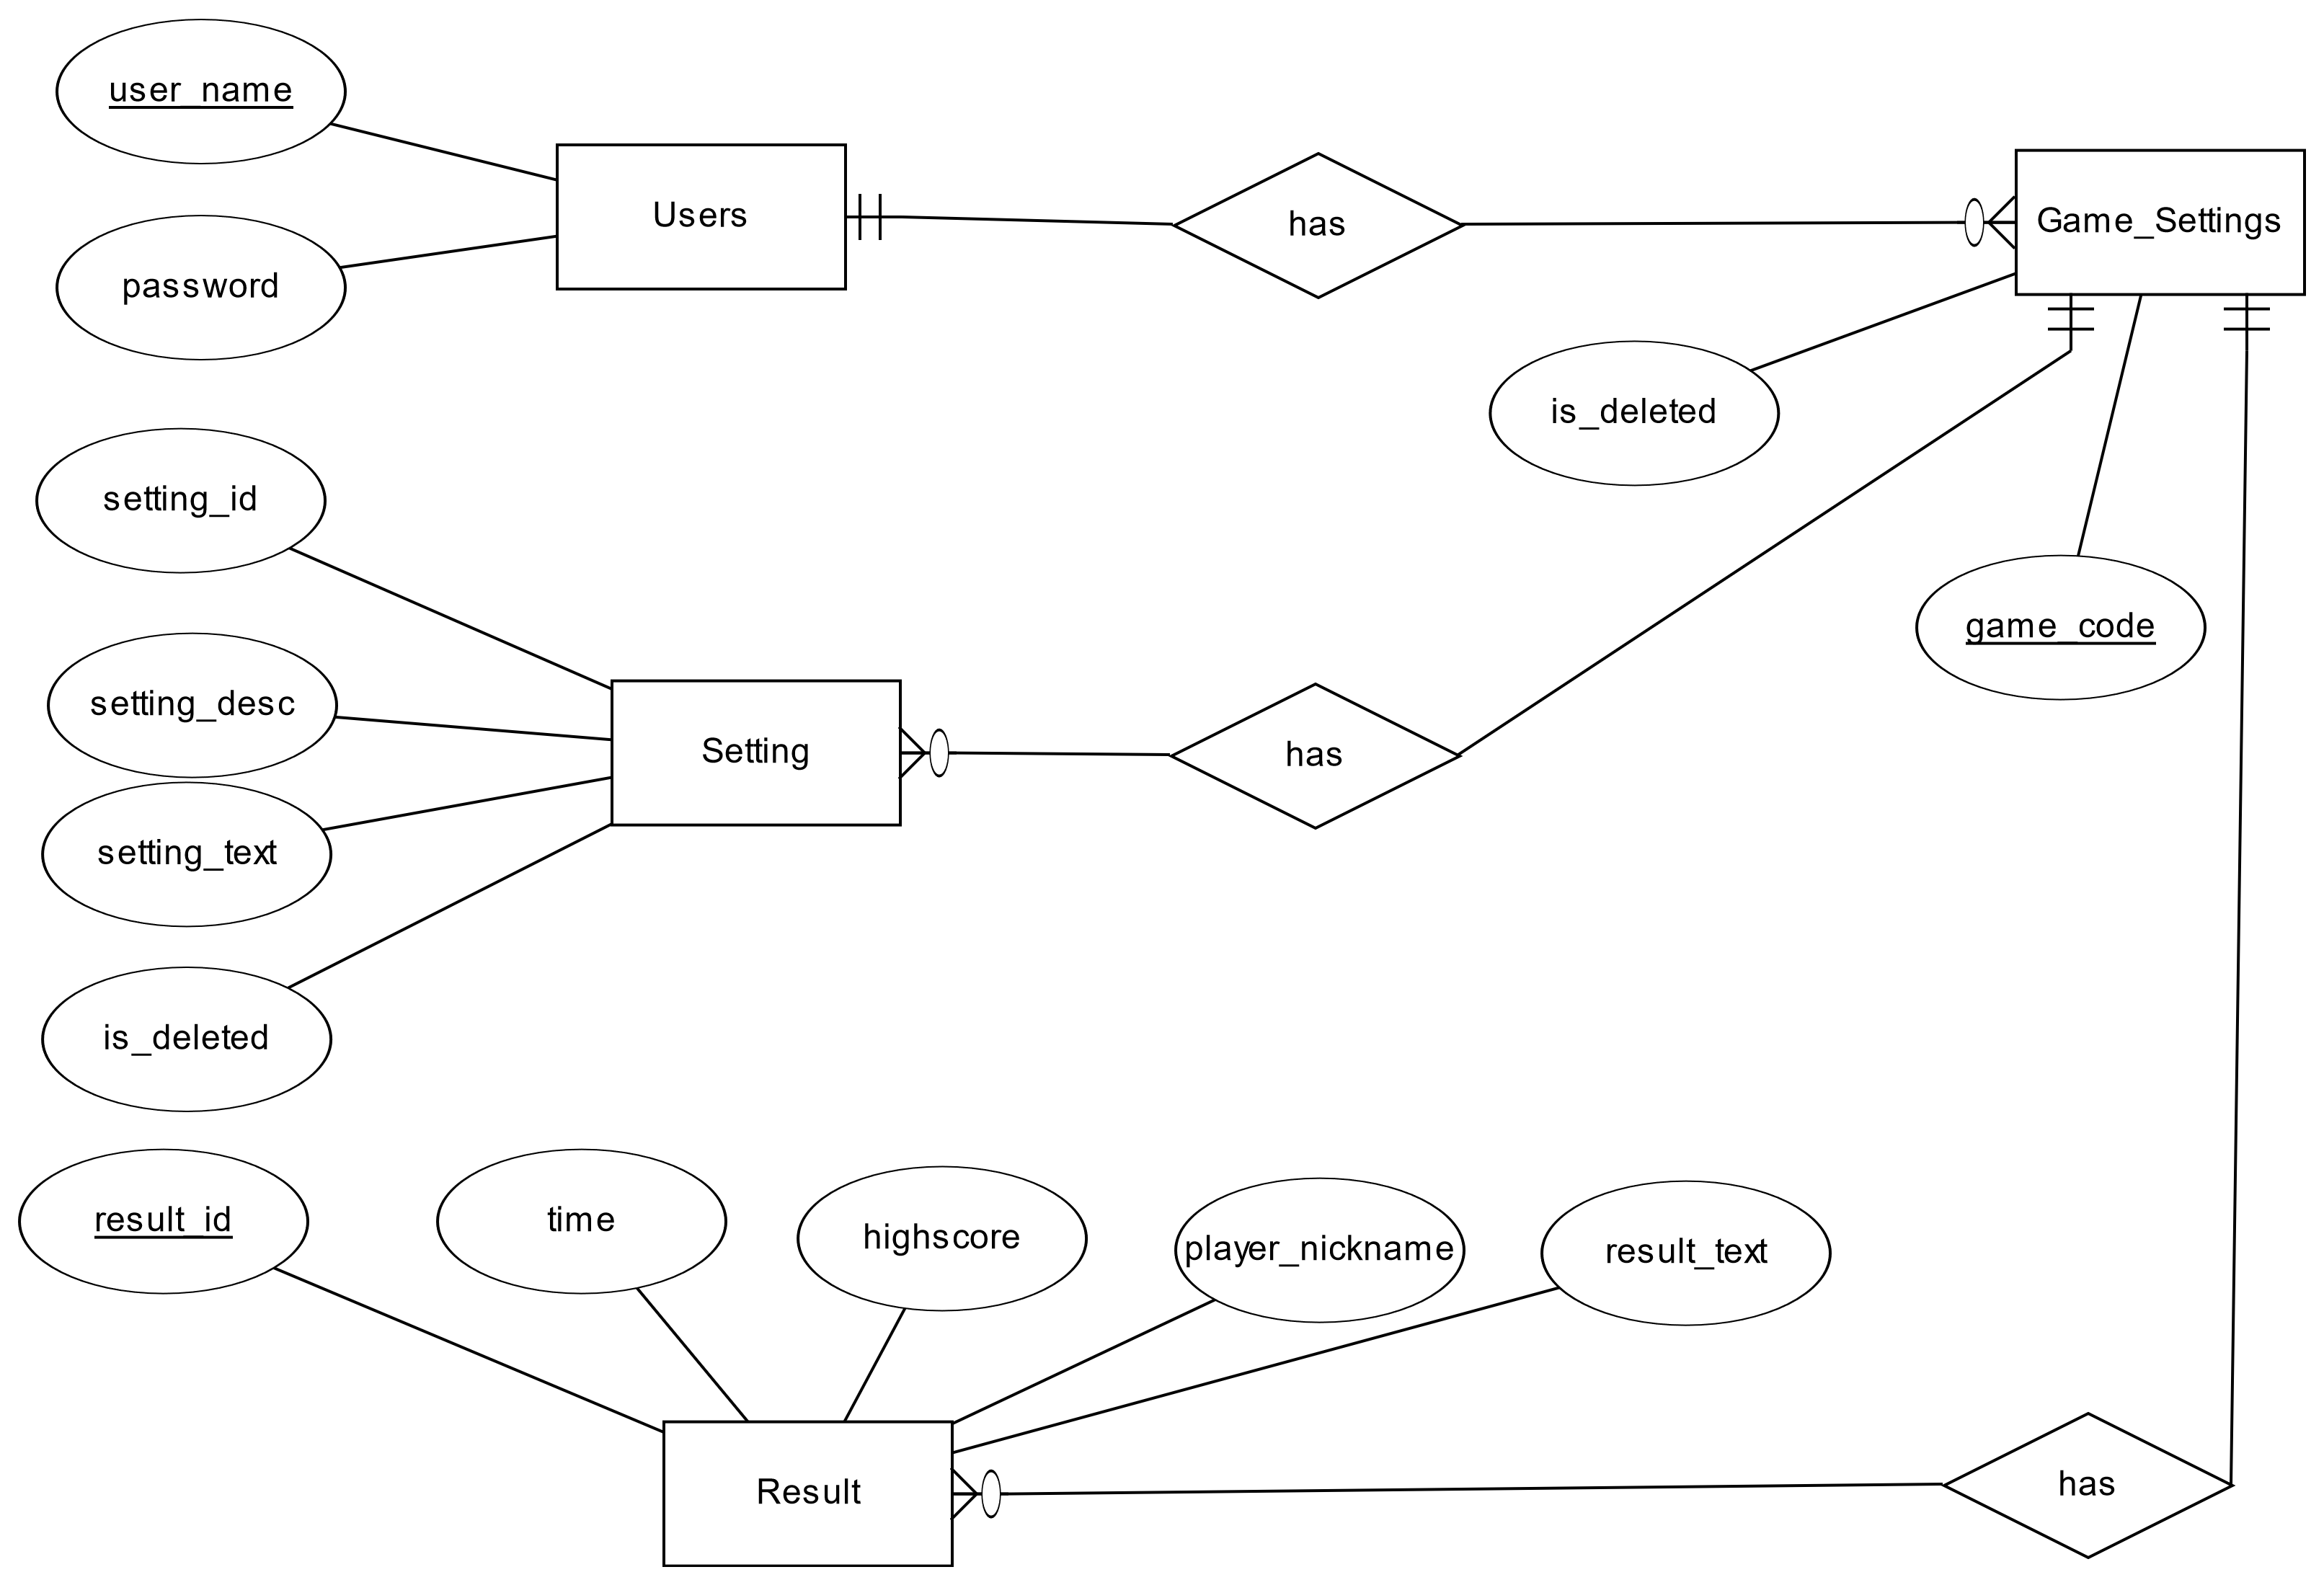
\includegraphics[width=\linewidth]{"slike/ER.png"} 
			\centering
			\caption{ER dijagram baze podataka}
			\label{fig:erdijagram}
		\end{figure}

	
	\section{Opis entiteta i tablica}
			\textbf {Users} \hspace{5mm}
			{Ovaj entitet označava korisnika koji koristi web aplikaciju, odnosno web sučelje za učitelja. Sadrži atribute: user\_ name i password.
			Atribut user\_ name predstavlja korisničko ime korisnika, dok atribut password označava zaporku koja se ne sprema u "plain-textu", već kao 
			rezultat hash funkcije.
			Ovaj entitet u vezi je \textit{One-To-Many} s entitetom Game\_ Settings preko atributa user\_name.}
				
				\begin{longtblr}[
					label=none,
					entry=none
					]{
						width = \textwidth,
						colspec={|X[6,l]|X[6, l]|X[20, l]|}, 
						rowhead = 1,
					} %definicija širine tablice, širine stupaca, poravnanje i broja redaka naslova tablice
					\hline \multicolumn{3}{|c|}{\textbf{Users}}	 \\ \hline[3pt]
					\SetCell{LightGreen}user\_name & VARCHAR	&  	jedinstveni naziv korisnika  	\\ \hline
					password	& VARCHAR &  rezultat hash funkcije nad zaporkom 	\\ \hline 
				\end{longtblr}



			\textbf {Game\_ Settings} \hspace{5mm}
			{Ovaj entitet označava jedan "game room". Sadrži atribute: game\_ code i is\_ deleted.
			Ovaj entitet u vezi je \textit{Many-To-One} s entitetom Users preko atributa user\_ name, u vezi \textit{One-To-Many} s
			entitetom Setting preko atributa game\_ code te u vezi \textit{One-To-Many} s entitetom Result preko atributa game\_ code.}
				
				\begin{longtblr}[
					label=none,
					entry=none
					]{
						width = \textwidth,
						colspec={|X[6,l]|X[6, l]|X[20, l]|}, 
						rowhead = 1,
					} 
					\hline \multicolumn{3}{|c|}{\textbf{Game\_ Settings}}	 \\ \hline[3pt]
					\SetCell{LightGreen}game\_ code & INT	&  	jedinstveni idenfitikator game\_ settings   	\\ \hline
					is\_ deleted & INT & zastavica koja govori jesu li "game room" obrisan \\ \hline
					\SetCell{LightBlue}user\_ name & VARCHAR & oznaka korisnika kojem "game room" pripada \\ \hline
				\end{longtblr}


			\textbf {Setting} \hspace{5mm}
			{Ovaj entitet označava jedanu postavku. Sadrži atribute: setting\_ id, setting\_ desc, setting\_ text i is\_ deleted.
			Ovaj entitet u vezi je \textit{Many-To-One} s entitetom Game\_ Settings preko atributa game\_ code.}
				
				\begin{longtblr}[
					label=none,
					entry=none
					]{
						width = \textwidth,
						colspec={|X[6,l]|X[6, l]|X[20, l]|}, 
						rowhead = 1,
					} 
					\hline \multicolumn{3}{|c|}{\textbf{Setting}}	 \\ \hline[3pt]
					\SetCell{LightGreen}setting\_ id & INT	&  	jedinstveni idenfitikator za Setting  	\\ \hline
					setting\_desc & VARCHAR & tekst koji opisuje cilj zadatka \\ \hline
					setting\_text & VARCHAR & postavka formatirana tako da bude razumljiva mobilnoj igri \\ \hline
					is\_ deleted & INT & zastavica koja govori je li postavka obrisana \\ \hline
					\SetCell{LightBlue}game\_code & INT & oznaka Game\_Settings kojem Setting pripada \\ \hline
					
				\end{longtblr}
				
			
			\textbf {Result} \hspace{5mm}
			{Ovaj entitet označava jedan rezultat igranja igre na mobitelu uz preuzete postavke.
			Sadrži atribute: result\_ id, time, highscore, player\_ nickname te result\_ text.
			Ovaj entitet u vezi je \textit{Many-To-One} s entitetom Game\_ Settings preko atributa game\_ code.}
				
				\begin{longtblr}[
					label=none,
					entry=none
					]{
						width = \textwidth,
						colspec={|X[6,l]|X[6, l]|X[20, l]|}, 
						rowhead = 1,
					} 
					\hline \multicolumn{3}{|c|}{\textbf{Result}}	 \\ \hline[3pt]
					\SetCell{LightGreen}result\_ id & INT	&  	jedinstveni idenfitikator za Result  	\\ \hline
					time & VARCHAR & vrijeme pohrane rezultata u bazu podatka \\ \hline
					highscore & VARCHAR & ostvareni rezultat na igri  \\ \hline
					player\_ nickname & VARCHAR & nadimak igrača  \\ \hline
					result\_text & VARCHAR & JSON polje s događajima igre  \\ \hline
					\SetCell{LightBlue}game\_code & INT & oznaka Game\_Settings kojem Result pripada \\ \hline
					
				\end{longtblr}

	\newpage
	\section{Relacijski dijagram}
		Sljedeća slika prikazuje relacijski dijagram baze podataka.
		\begin{figure}[H]
			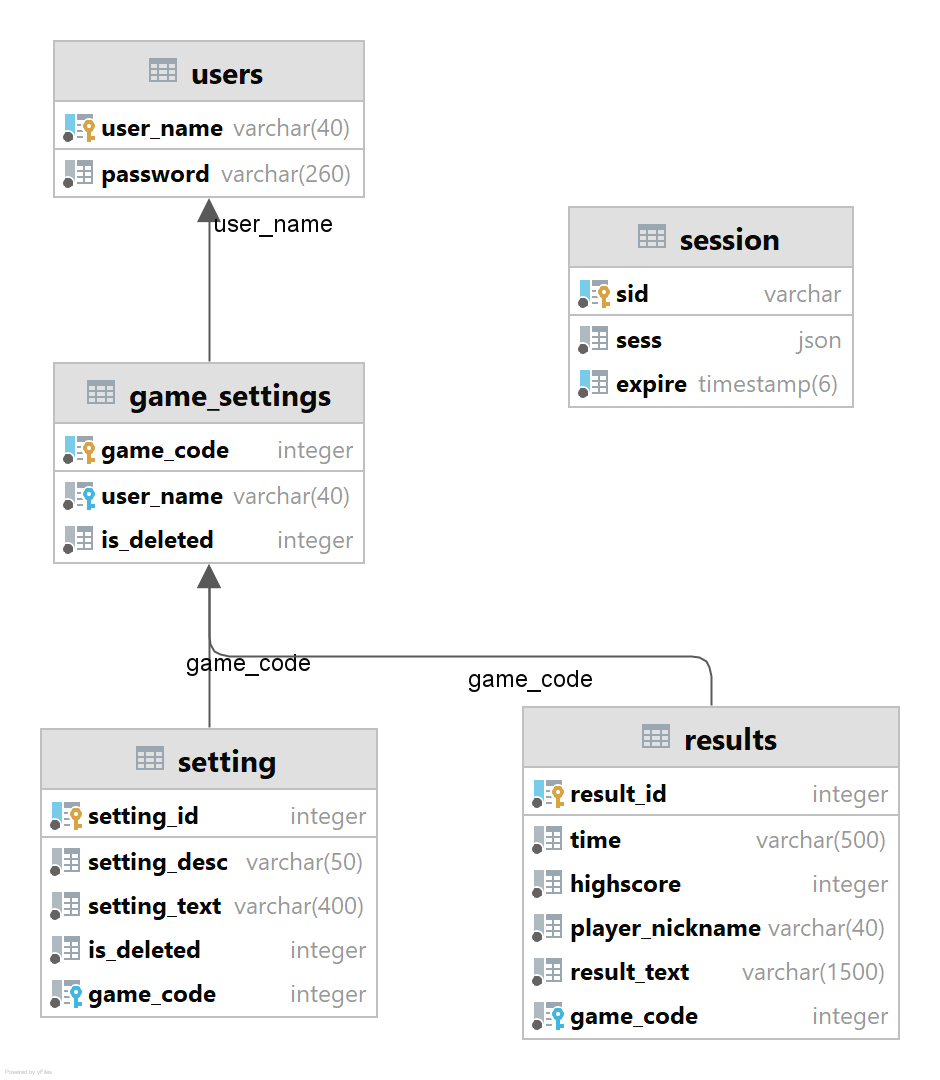
\includegraphics[width=\linewidth]{"slike/REL.png"} 
			\centering
			\caption{Relacijska shema baze podataka}
			\label{fig:relshema}
		\end{figure}


\chapter{Moguće nadogradnje}
Kao nadogradnju na učinjeno, odnosno budući rad postoji mnogo opcija. Za početak prilagodba web stranice kako bi se prilagodila mobilnim uređajima, nadalje dodavanje raznih animacija u igru, izrada priče, skupljanje novčića
i otključavanje raznih stvari poput novih motiva pozadine, objekta s kojim se skupljaju padajući objekti i slično, generalno postojanje nekog tipa napretka koji bi potaknuo korisnike na češću uporabu aplikacije.
Nažalost, mobilnu igru nije koristila ciljana skupina ljudi, odnosno učenici nižih razreda osnovne škole stoga je teško procijeniti da li je algoritam napravljen za prilagodbu u potpunosti dobar, u najboljem slučaju potreban
je neki tip kalibracije. 

\chapter{Zaključak}
U skolopu ovog završnog rada razvijena je mobilna igra za vježbanje matematike koja se težinom prilagođava igraču  i web stranica koja omogućava jednostavnu izradu
postavki igre i detaljni pregled rezultata pojedinog učenika u nekoj igri. Za potrebe pohrane podataka koristi se lokalni spremnik na samom uređaju pa tako i baza podataka kojoj se pristupa preko poslužitelja.
Ovaj projekt kao takav nije zahtjevao previše specifičnih znanja već samo osnove objektno orijentiranog programiranja, osnove pisanja web stranica i poslužitelja te osnovna znanja iz baza podataka. Shodno tome nije bilo 
potrebe za istraživanjem različitih algoritama, već se većina toga svela na oblikovanje ideje igre te mukotrpan i vremenski zahtjevan posao. No, u konačnici kroz ovaj projekt upoznao sam se sa izradom mobilnih aplikacija 
i dobio dobru praksu u korištenju raznih tehnologija.


\bibliography{literatura}
\bibliographystyle{fer}

\begin{sazetak}
U skolopu ovog završnog rada razvijena je mobilna igra za vježbanje matematike koja se težinom prilagođava igraču  i web stranica koja omogućava jednostavnu izradu
postavki igre i detaljni pregled rezultata pojedinog učenika u nekoj igri. Navedena igra i web stranice čine jedan jednostavni sustav. Unutar ovog rada detaljno je opisano što ovaj sustav sve nudi te su također opisani
i najznačajniji implementacijski detalji.

\kljucnerijeci{Java, Android, igra, matematika, web stranica, HTML, Node.js, Express.js, JavaScript, vježba, učenje, igrifikacija, škola}
\end{sazetak}

% TODO: Navedite naslov na engleskom jeziku.
\engtitle{Mobile game for practicing math}
\begin{abstract}
As part of this thesis, there've been developed mobile game for practicing mathematics that is adaptive to the player's abilities and a website that allows easy creation of game settings and a detailed overview of
the results of each student in a game. Mentioned game and website make one simple system. Within this paper it is described what this system offers in details just like the most important implementation details.

\keywords{Java, Android, game, math, web page, HTML, Node.js, Express.js, Javascript, exercise, learning, gamification, school}
\end{abstract}

\end{document}
